% Insert result section here. 
\section{Results}
\label{sec:Results}
The results are split into subsections depending on the type of CP Violation allowed.
Additonally, results are presented using a variety of different combinations of the
available data. Figure~\ref{fig:xy_nocpv_variations} shows all variations for the 
no CPV allowed fits. Figure~\ref{fig:xy_all_variations} shows the results for a 
subset of variations on All CPV allowed fits. 
\subsection{No CP Violation Allowed}
Table~\ref{table:nocpv_output_table} lists the results from the No CP Violation allowed
global fit. As $A_\Gamma =0$ in the the case of No CPV, the data is not included in 
this fit. Additionally, we take subsets of the data which do not include results from
Belle, BaBar and CDF in order to explore the change in $\chi^2/$ndf of the global fit.
\begin{table}[htdp]
%	\begin{scriptsize}

\begin{center}
\resizebox{16cm}{!}{
\begin{tabular}{|c||c||c||c||c|}
\hline
 & All Results & No BaBar $K\pi$& No Belle, BaBar $K\pi$ & No Belle, BaBar, CDF $K\pi$ \\ \hline
$x[\%]                    $ & $0.378\pm 0.180 $& $0.467\pm 0.183  $& $0.473\pm 0.186  $& $0.474\pm 0.187$ \\ \hline
$y[\%]                    $ & $0.629\pm 0.080 $& $0.649\pm 0.089  $& $0.651\pm 0.090  $& $0.655\pm 0.090$ \\ \hline
$\delta_{K\pi}[\text{deg}]$ & $9.334\pm 12.487$& $14.601\pm 10.694$& $14.902\pm 10.689$& $14.550\pm 10.730$ \\ \hline
$R_D[10^{-3}]             $ & $3.493\pm 0.039 $& $3.542\pm 0.044  $& $ 3.547\pm 0.047 $& $3.547 \pm 0.047$ \\ \hline
$\chi^2/ndf               $ & $43.8487/16     $& $27.8873/13      $& $24.343/10       $& $13.5119/7$ \\ \hline
\end{tabular}
}
\end{center}
\caption{Output values of No CPV allowed global fit. Different columns list subsets of
allowed data.}
\label{table:nocpv_output_table}
%\end{scriptsize}
\end{table}%

\begin{figure}[htb]
  \begin{center}
    \begin{subfigure}[b]{0.4\textwidth}
      \centering
      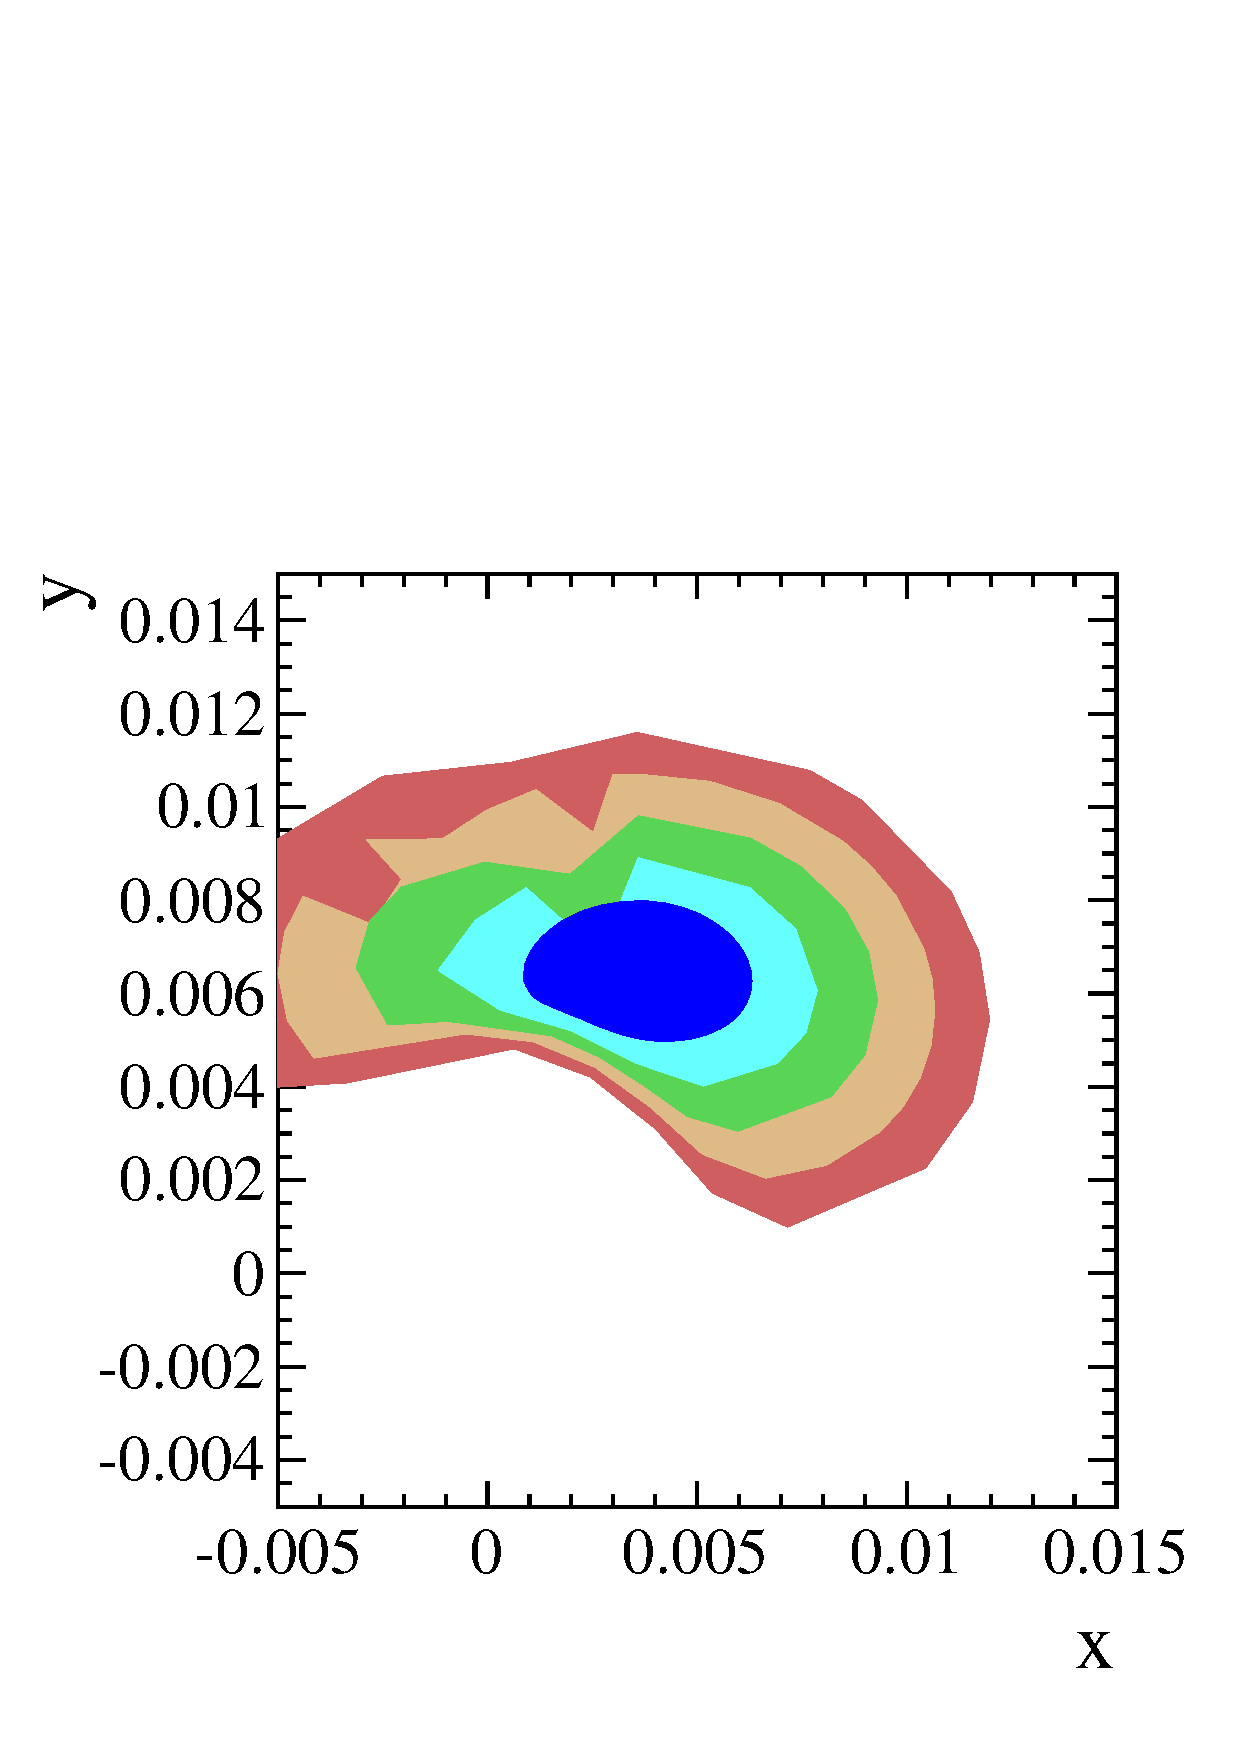
\includegraphics[width=\textwidth]{finalplot_nocpv__graph.pdf}
      \caption{Two dimensional error ellipses for x and y using all measurements listed in Table~\ref{table:nocpv_output_table}.}
      \label{fig:xy_no_cpv_}
    \end{subfigure}\hspace{3mm}%
    \begin{subfigure}[b]{0.4\textwidth}
      \centering
      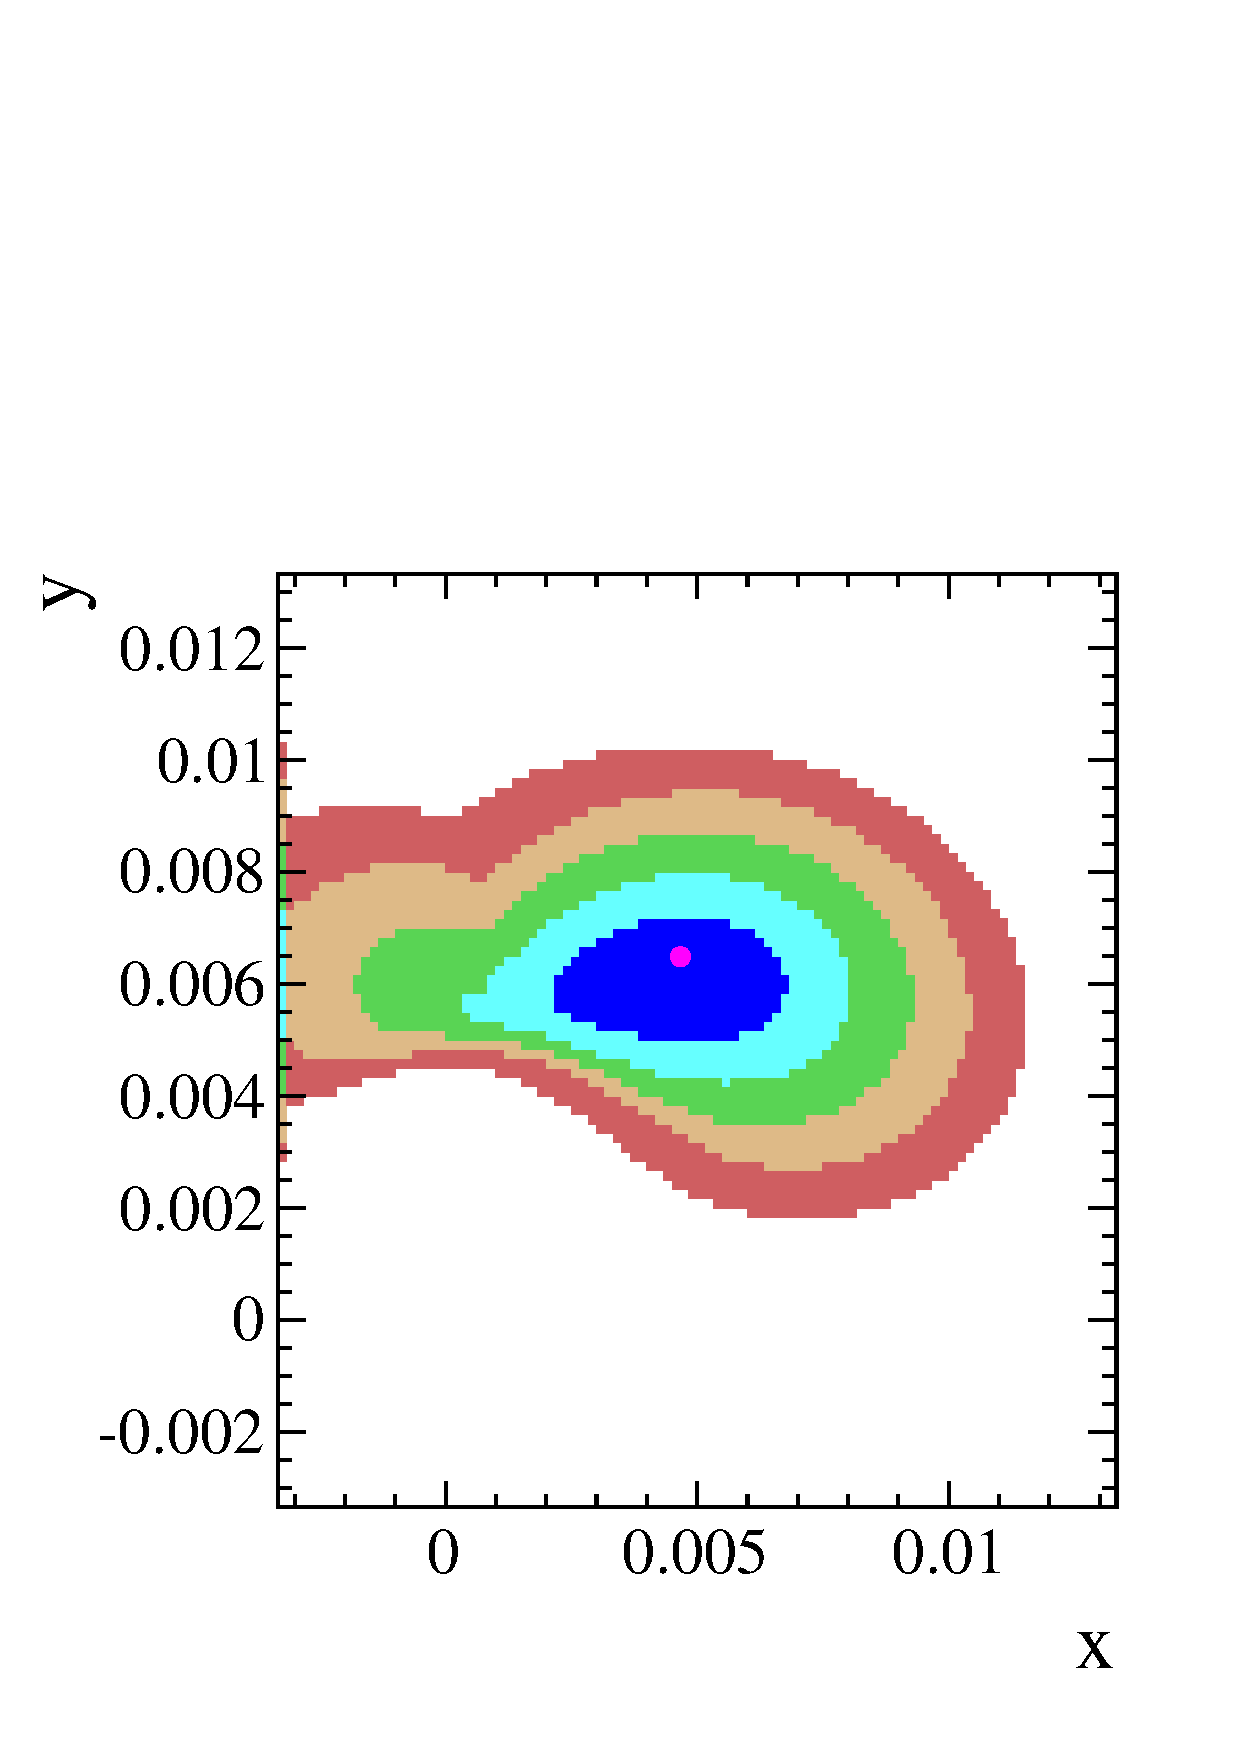
\includegraphics[width=\textwidth]{finalplot_nocpv__babar_graph.pdf}
      \caption{Two dimensional error ellipses for x and y using all available measurements except the BaBar $K\pi$ measurements.}
      \label{fig:xy_no_cpv_no_babar}
    \end{subfigure}%
    %\hspace{2mm}
    
    \begin{subfigure}[b]{0.4\textwidth}
      \centering
      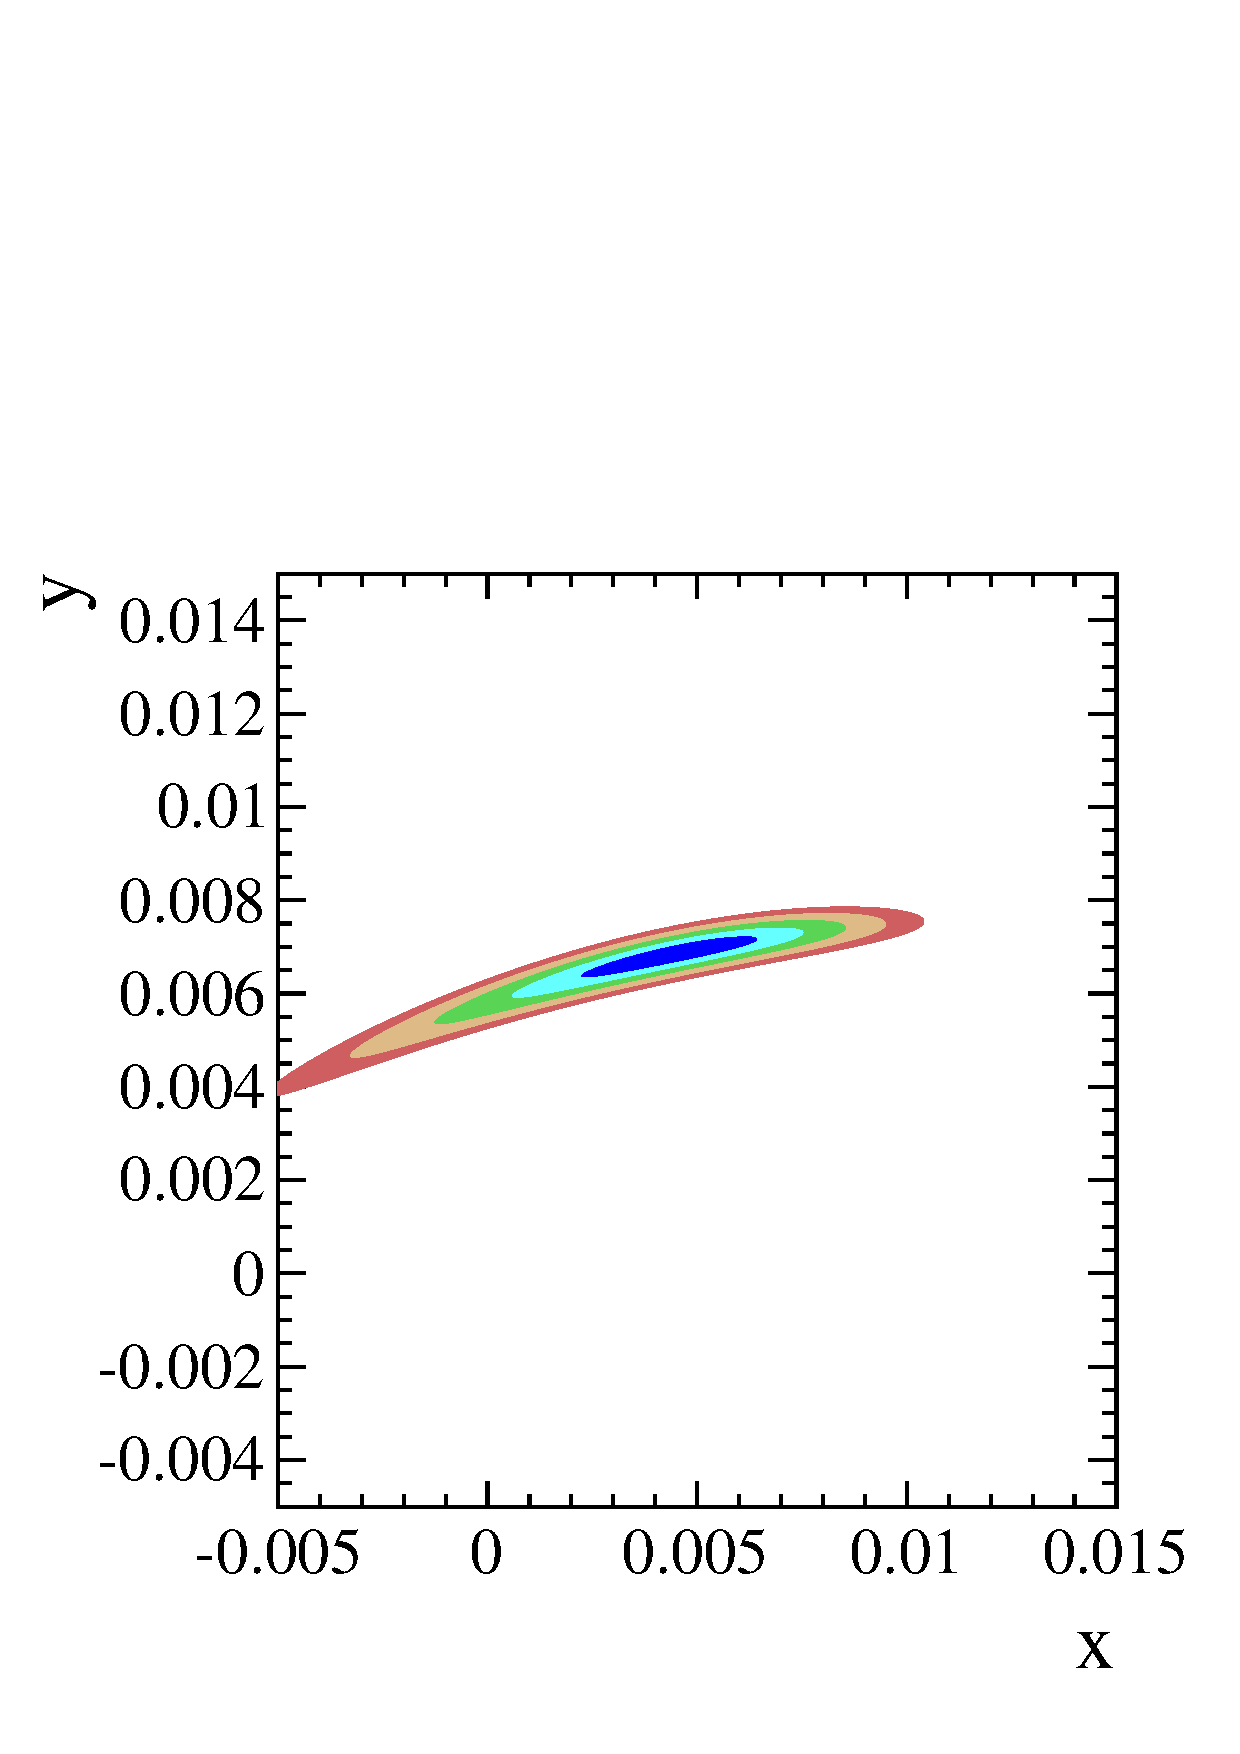
\includegraphics[width=\textwidth]{finalplot_nocpv__belle_babar_graph.pdf}
      \caption{Two dimensional error ellipses for x and y from fit excluding Belle and BaBar $K\pi$ results.}
      \label{fig:xy_no_cpv_nobelle_babar}
    \end{subfigure}%
    \hspace{2mm}
    \begin{subfigure}[b]{0.4\textwidth}
      \centering
      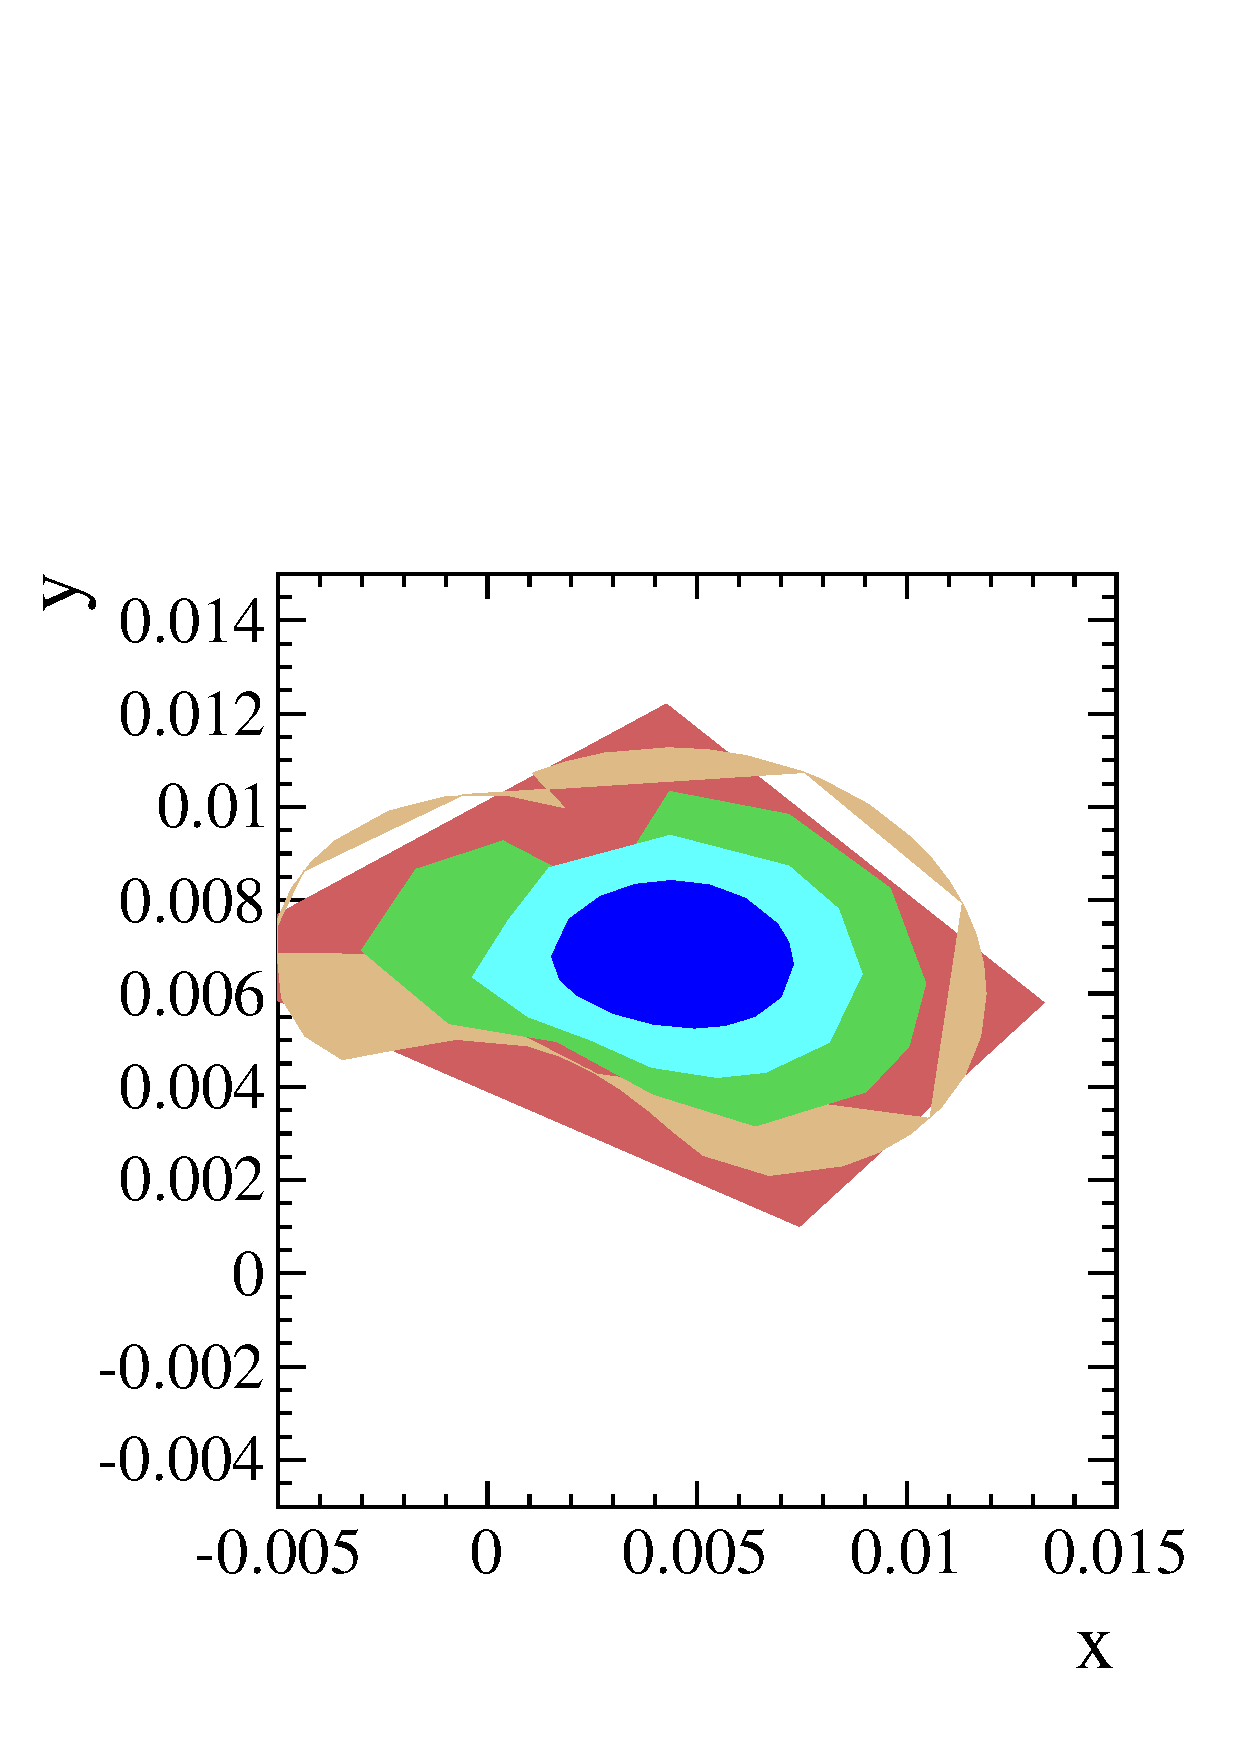
\includegraphics[width=\textwidth]{finalplot_nocpv__belle_babar_cdf_graph.pdf}
      \caption{Two dimensional error ellipses for x and y from fit excluding Belle, BaBar and CDF measurements.}
      \label{fig:xy_no_cpv_nocdf}
    \end{subfigure}%
    %\vspace*{-1.0cm}
  \end{center}
  \caption{Two dimensional error ellipses of $x$ and $y$ from fit for No CPV. Exclusion of the Belle and BaBar results drastically change the slope of the error ellipses. The differing colors represent the 1-5$\sigma$ contours.}
  \label{fig:xy_nocpv_variations}
\end{figure}


\subsection{No Direct CP Violation Allowed}
As opposed to the No CP violation case, allowing CP violation excepting direct CP Violation
allows the inclusion of additional global results. For instance, the preliminary result 
for $A_\Gamma$ from $KK$ and $\pi\pi$ as reported by LHCb
Table~\ref{table:nodcpv_output_table_no_lhcb_agamma} lists the results of the global fit without direct
CP violation, but excluding the preliminary LHCb $A_\Gamma$ results.
The complementary results including the LHCb $A_\Gamma$ results are listed in
Table~\ref{table:nodcpv_output_table_with_lhcb_agamma}.
The inlcusion of this result does not change the central values or errors substantially. 
Additionally, in all cases, the error on $|q/p|$ is of order 1.3\%.\\
As described in Section~\ref{sec:fit_variants}, it is possible to inverte the relationship
 between $|q/p|$ and $\phi$ to instead fit for $\phi$ as the free parameter in the fit. 
Table~\ref{table:nodcpv_output_table_no_lhcb_agamma_phi} lists the results of this fit 
excluding the preliminary LHCb $A_\Gamma$ result, and Table~\ref{table:nodcpv_output_table_with_lhcb_agamma_phi} 
lists the results including the preliminary result.


\begin{table}[htdp]
%\begin{tiny}

\begin{center}
\resizebox{16cm}{!} {
\begin{tabular}{|c||c||c||c||c|}
\hline
& All Measurements & No Belle, BaBar$K\pi$& No Belle, BaBar$K\pi$, add $A_{\Gamma\text{ LHCb}}$ & No Belle, BaBar, CDF $K\pi$, add $A_{\Gamma\text{ LHCb}}$ \\ \hline

$x(\times10^{-3})$ & $ 5.191\pm 1.746 $& $4.843\pm 1.782$& $4.845\pm1.782$& $4.844\pm1.787$ \\ \hline

$y(\times10^{-3})$ &$ 6.343\pm 0.905$ & $6.797\pm 1.029$& $6.797\pm 1.030$& $6.809\pm 1.031$ \\ \hline

$\delta_{K\pi}(\times10^{-1})[\text{rad}]$ &$2.468\pm 1.763$ & $3.187\pm 2.021$&$3.188\pm 2.021$ & $3.084\pm 2.040$ \\ \hline

$R_D(\times10^{-3})$ & $ 3.571\pm 0.046 $&$3.555\pm0.046$ & $3.556\pm 0.046$& $3.556\pm 0.047$ \\ \hline

$|q/p|(\times10^{-1})$ & $9.931 \pm 0.125$& $9.935\pm0.135$& $9.929\pm 0.131$ & $9.930\pm0.130 $\\ \hline

$\chi^2/ndf$ & 24.8569/28 & 19.0559/13& 19.3925/15& 8.61793/12\\ \hline

\end{tabular}
}
\end{center}
\caption{Output values of No Direct CPV allowed global fit. Different columns list 
subsets of allowed data.}
\label{table:nodcpv_output_table}
%\end{tiny}
\end{table}%



\begin{table}[htdp]
%\begin{tiny}

\begin{center}
\resizebox{16cm}{!} {
\begin{tabular}{|c||c||c||c||c|}
\hline
& All Measurements & No BaBar$K\pi$& No Belle, BaBar $K\pi$ & No Belle, BaBar, CDF $K\pi$ \\ \hline

$x[\%]                    $ &$0.534\pm 0.173 $ &$0.533\pm 0.174 $ &$0.503\pm 0.174  $ & $0.501\pm 0.175$ \\ \hline

$y[\%]                    $ &$0.655\pm 0.093 $ &$0.656\pm 0.092 $ &$0.649\pm 0.091  $ & $0.652\pm 0.090$ \\ \hline

$\delta_{K\pi}[\text{deg}]$ &$16.506\pm 9.752$ &$16.268\pm 9.805$ &$14.644\pm 10.341$ & $14.170\pm 10.429$\\ \hline

$R_D[10^{-3}]             $ &$3.578\pm 0.047 $ &$3.571\pm 0.047 $ &$3.551\pm 0.046  $ & $3.551\pm 0.047$ \\ \hline

$\phi[\text{deg}]         $ &$0.286\pm 0.590 $ &$0.2784\pm 0.590$ &$0.284\pm 0.593  $ & $0.280\pm 0.587$ \\ \hline

$\chi^2/ndf               $ &$23.9035/26     $ &$28.1998/21     $ &$28.5592/16      $ &$17.723/13$ \\ \hline

\end{tabular}
}
\end{center}
\caption{Output values of No Direct CPV allowed global fit, with $|q/p|$ fixed.
These results exclude the preliminary LHCb $A_\Gamma$ results from the fit. 
Different columns list subsets of allowed data.}
\label{table:nodcpv_output_table_no_lhcb_agamma_phi}
%\end{tiny}
\end{table}%


\begin{table}[htdp]
%\begin{tiny}

\begin{center}
\resizebox{16cm}{!} {
\begin{tabular}{|c||c||c||c||c|}
\hline
& All Measurements & No BaBar$K\pi$& No Belle, BaBar $K\pi$ & No Belle, BaBar, CDF $K\pi$ \\ \hline

$x[\%]                    $ &$0.534\pm 0.173 $ &$0.533\pm 0.173 $ &$0.503\pm 0.174  $ &$0.502\pm 0.175$  \\ \hline

$y[\%]                    $ &$0.656\pm 0.093 $ &$0.656\pm 0.093 $ &$0.649\pm 0.091  $ &$0.652\pm 0.091$ \\ \hline

$\delta_{K\pi}[\text{deg}]$ &$16.519\pm 9.745$ &$16.268\pm 9.185$ &$14.644\pm 10.340$ &$14.241\pm 10.425$ \\ \hline

$R_D[10^{-3}]             $ &$3.579\pm 0.047 $ &$3.571\pm 0.047 $ &$3.551\pm 0.046  $ &$3.551\pm 0.0047$  \\ \hline

$\phi[\text{deg}]         $ &$0.315\pm 0.573 $ &$0.307\pm 0.573 $ &$0.312\pm 0.576  $ &$0.307\pm 0.569$ \\ \hline

$\chi^2/ndf               $ &$24.2399/28     $ &$28.5374/23     $ &$28.8959/18      $ &$18.0602/15$ \\ \hline

\end{tabular}
}
\end{center}
\caption{Output values of No Direct CPV allowed global fit, fixing
$|q/p|$ and fitting for $\phi$.
These results include the preliminary LHCb $A_\Gamma$ results in the fit. 
Different columns list subsets of allowed data.}
\label{table:nodcpv_output_table_with_lhcb_agamma_phi}
%\end{tiny}
\end{table}%

\begin{figure}[htb]
  \begin{center}
    \begin{subfigure}[b]{0.4\textwidth}
      \centering
      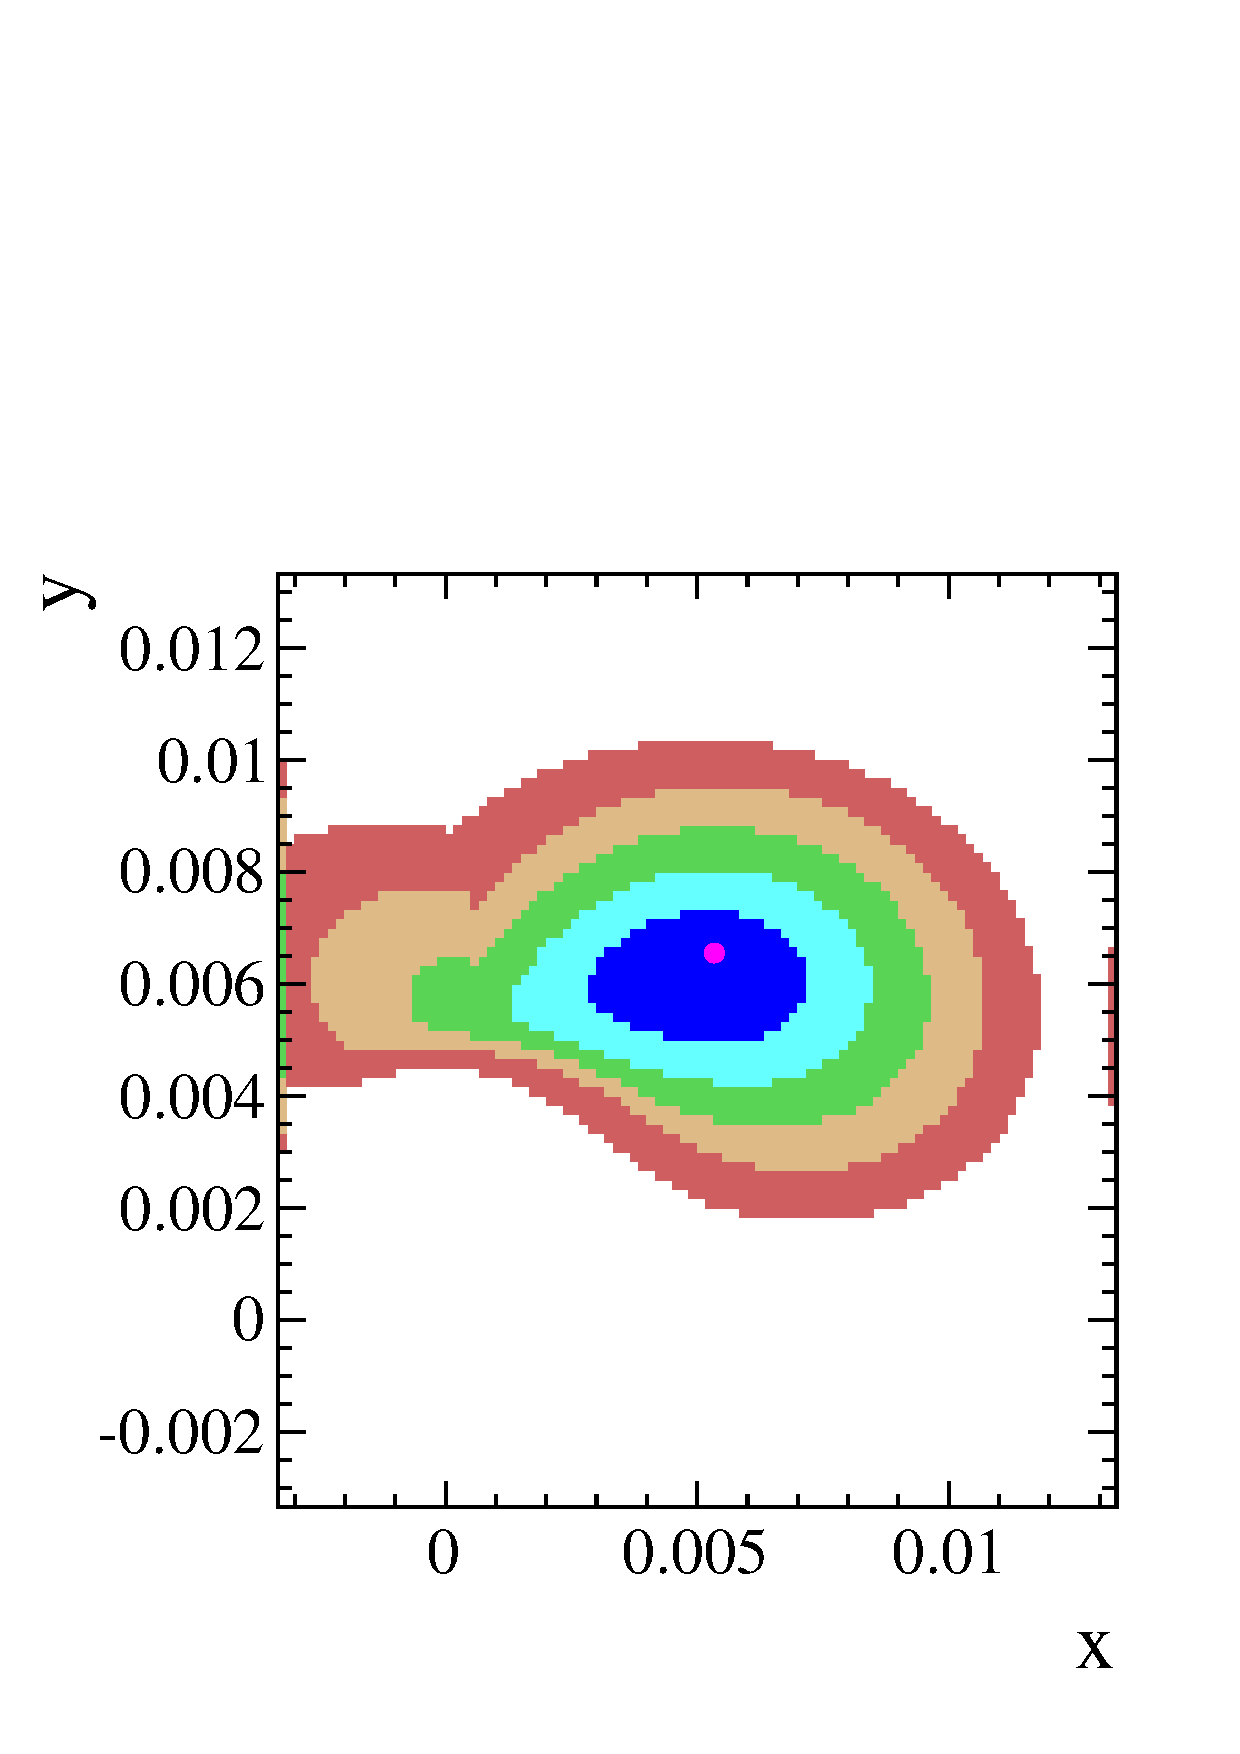
\includegraphics[width=\textwidth]{finalplot_nodcpv__.pdf}
      \caption{Two dimensional error ellipses for x and y from fit to all listed data.}
      \label{fig:all_nodcpv}
    \end{subfigure}%
    \hspace{2mm}
    \begin{subfigure}[b]{0.4\textwidth}
      \centering
      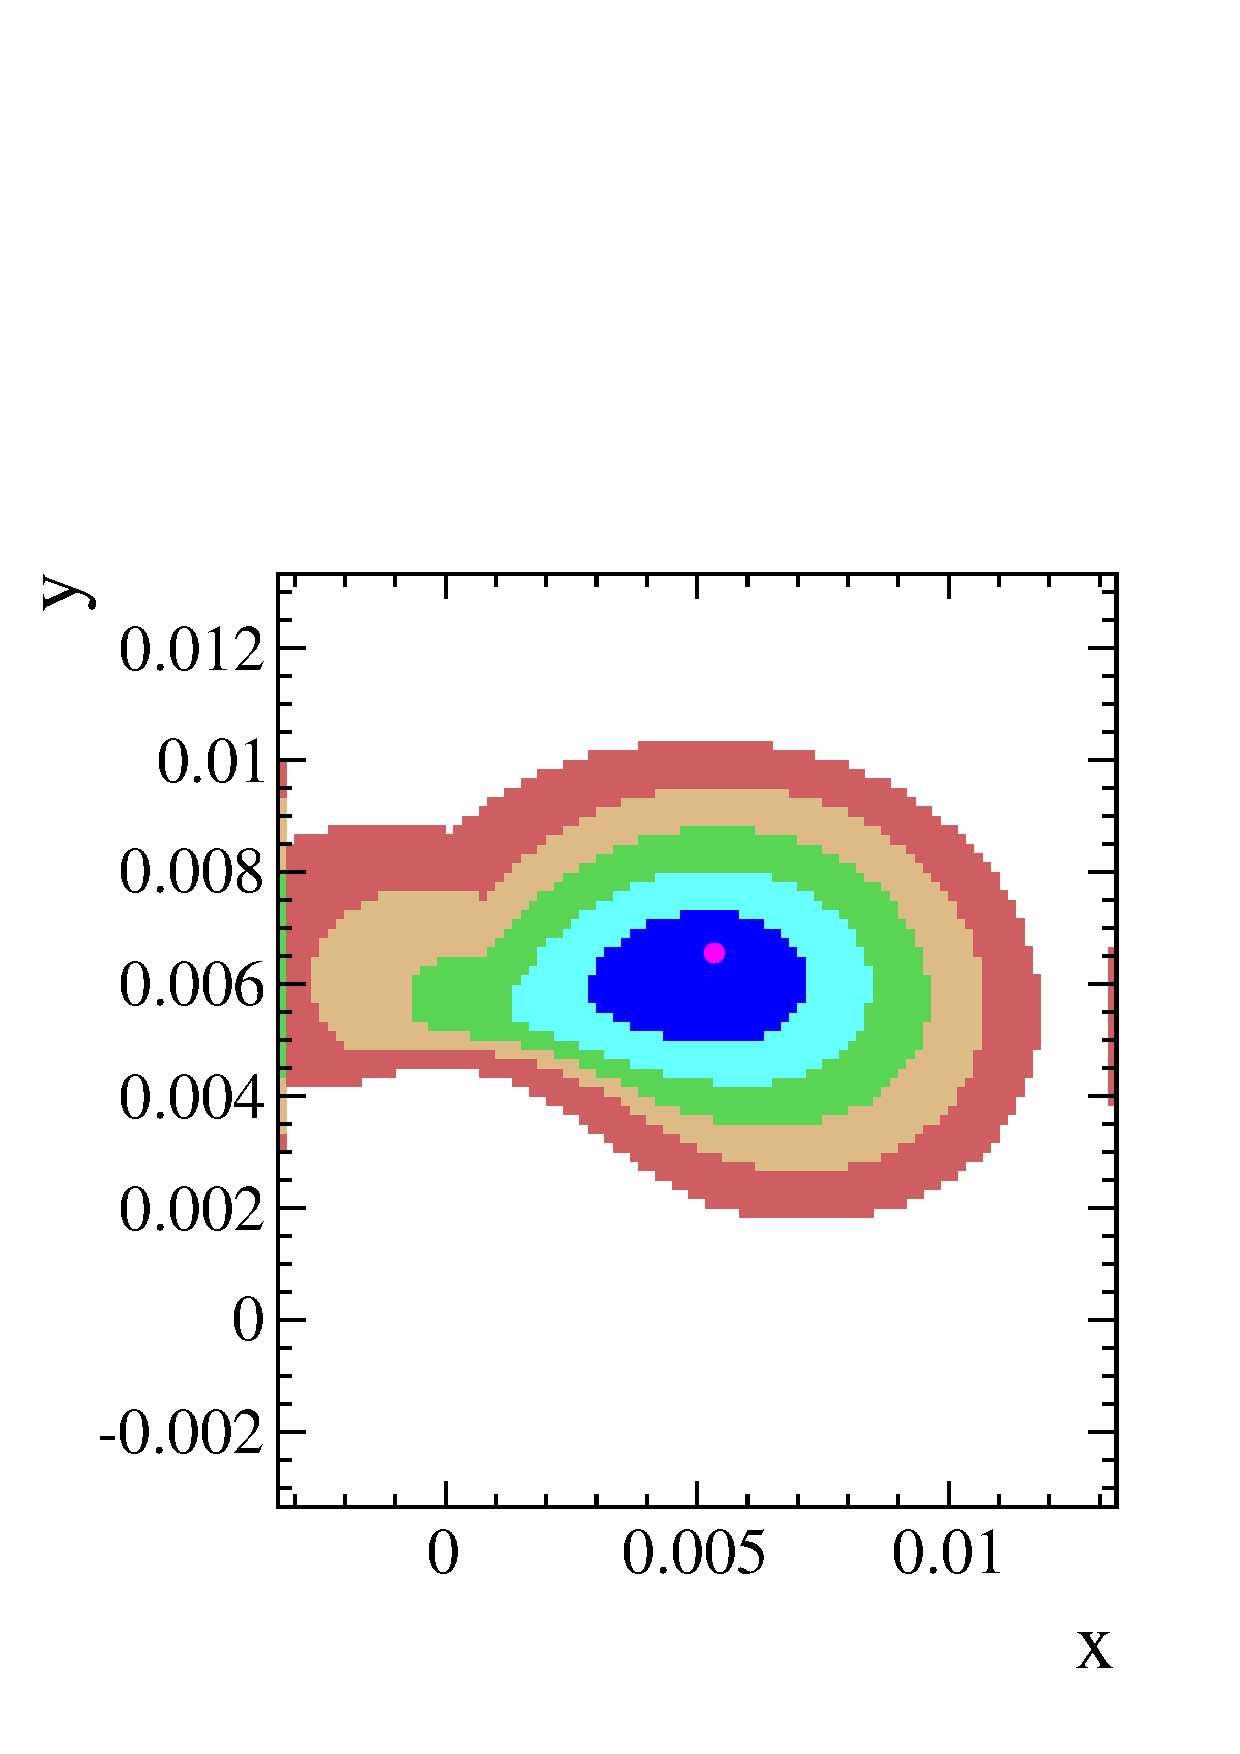
\includegraphics[width=\textwidth]{finalplot_nodcpv___hfag_agamma.pdf}
      \caption{Two dimensional error ellipses for x and y from fit to all data except LHCb $A_\Gamma$.}
      \label{fig:all_nodcpv_no_lhcb_agamma}
    \end{subfigure}%
    \\
%%%%%%%%%
    %\hspace{2mm}
    \begin{subfigure}[b]{0.4\textwidth}
      \centering
      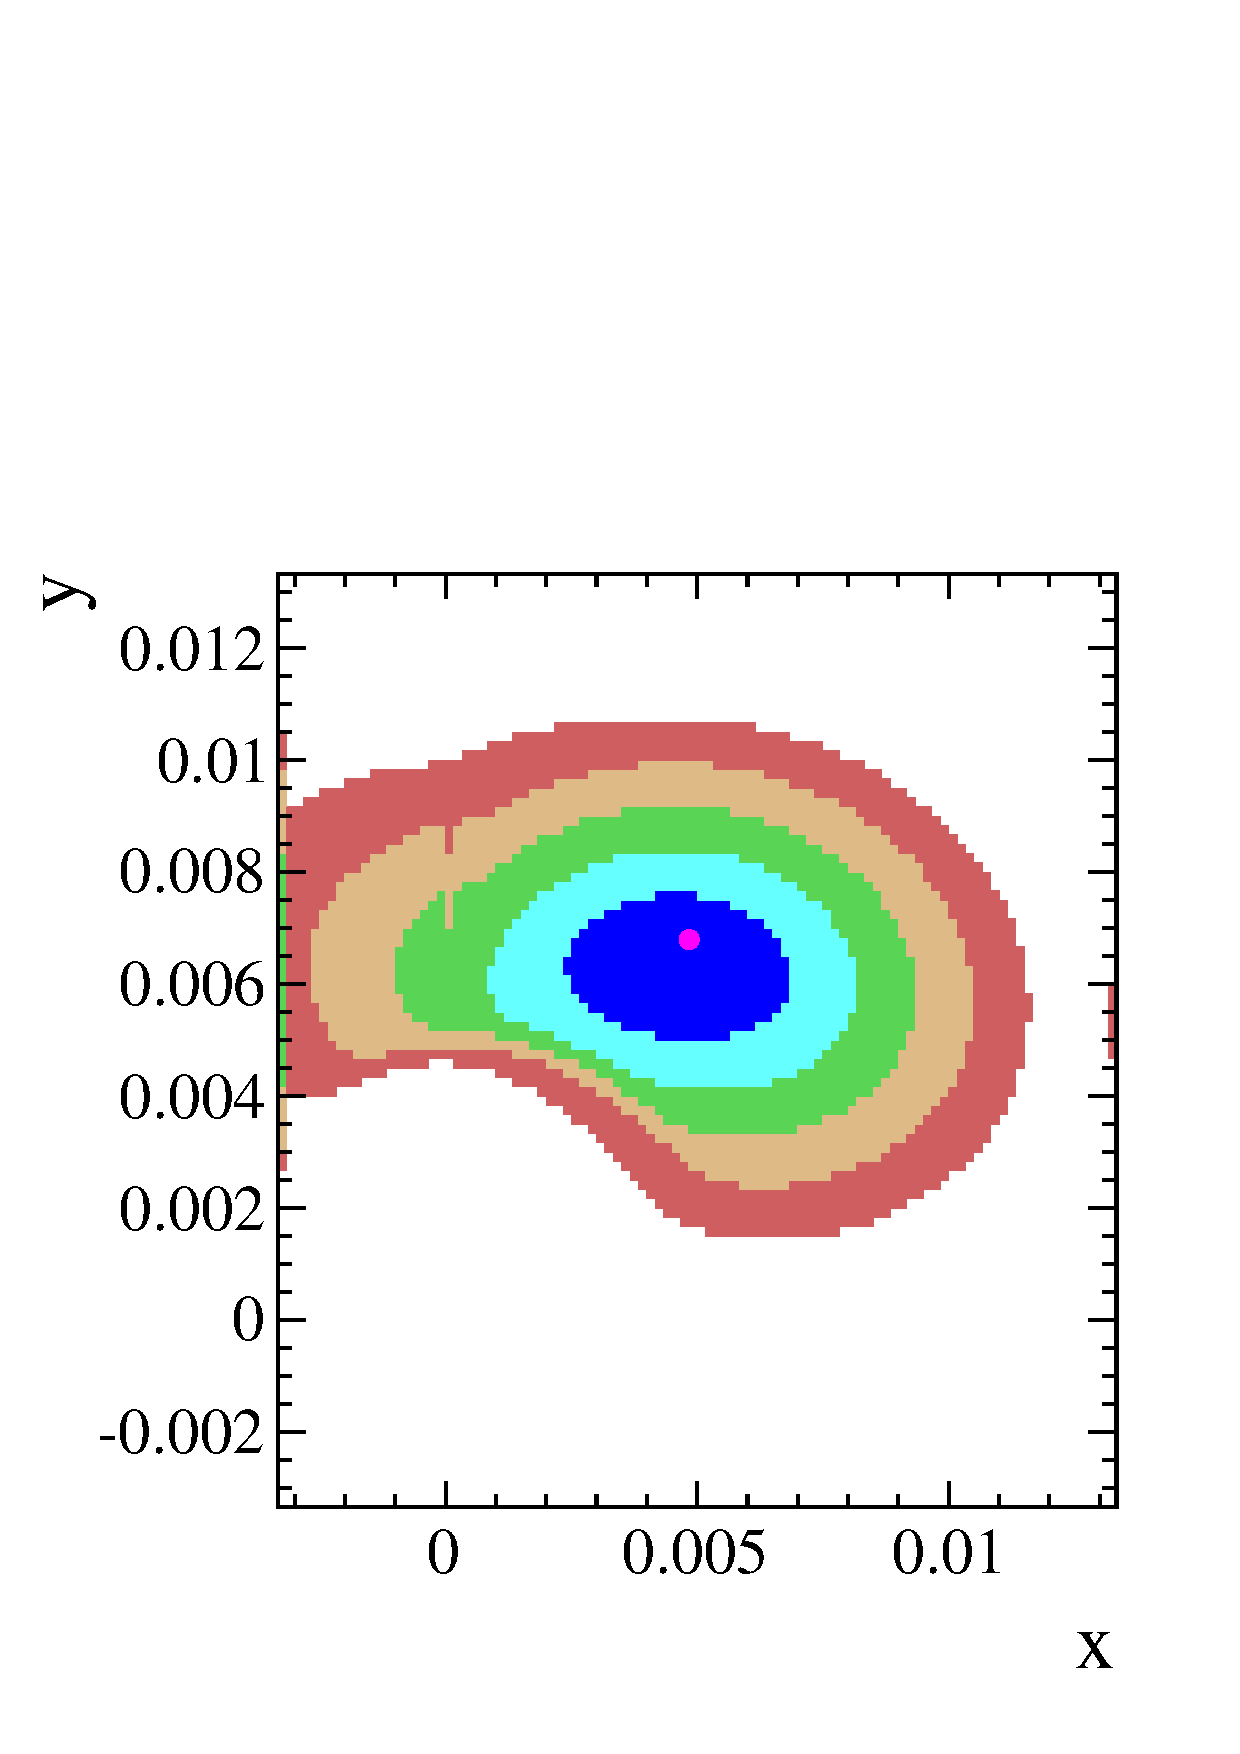
\includegraphics[width=\textwidth]{finalplot_nodcpv__nobelle_babar_.pdf}
      \caption{x vs y for Data excluding Belle and Babar $K \pi$ results.}
      \label{fig:nodcpv_no_belle_babar}
    \end{subfigure}%
    \hspace{2mm}
    \begin{subfigure}[b]{0.4\textwidth}
      \centering
      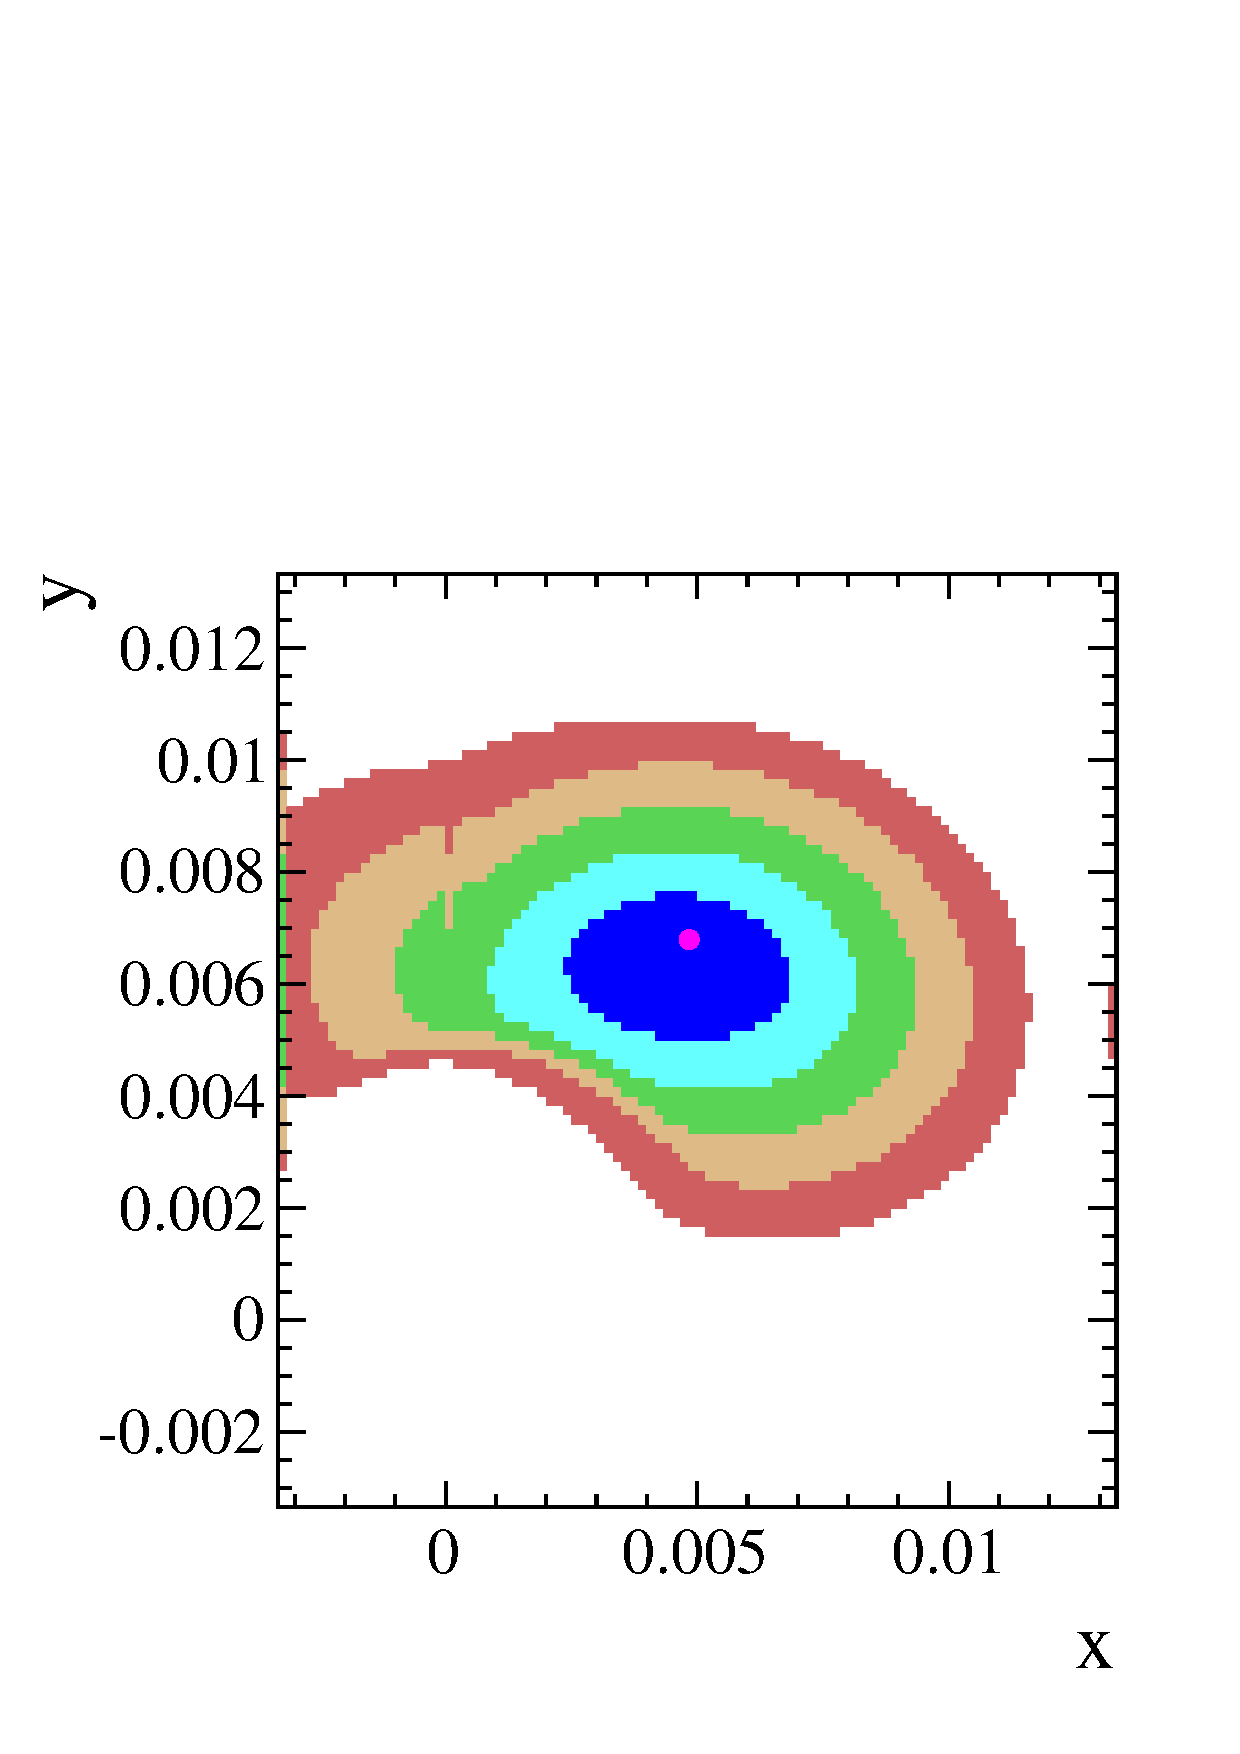
\includegraphics[width=\textwidth]{finalplot_nodcpv__nobelle_babar__hfag_agamma.pdf}
      \caption{Two dimensional error ellipses for x and y for No Direct CPV, excluding Belle and BaBar $K\pi$ results, and excluding LHCb $A_\Gamma$.}
      \label{fig:nodcpv_no_belle_babar_no_lhcb_agamma}
    \end{subfigure}%
    %\vspace*{-1.0cm}
  \end{center}
  \caption{Two dimensional error ellipses of fit for All CPV including differing sets of data for $x$ vs $y$. The biggest differences come from including the CDF result, which elongates the error ellipses. The differing colors represent the 1-5$\sigma$ contours.}
  \label{fig:xy_nodcpv_variations}
\end{figure}


%%%%%%%%%%%%%%%%%%%%%%%%%%%%%%%%%%%%%%%%%%%%
\subsection{All CP Violation Allowed}
Table~\ref{table:allcpv_output_table} lists the results of the global All CP Violation
allowed fit. Again, the latter columns list the differing subsets of the data to explore
the variation in global $\chi^2/$ndf. The most noticable difference between all fits
is the evaluation of $x$, which varies quite a bit with the inclusion of differing datasets.


%%%%%%%%%%%%%%% XY %%%%%%%%%%%%%%%%%%%%%%%%%
\begin{table}[htdp]
%\begin{tiny}

\begin{center}
\resizebox{16cm}{!} {
\begin{tabular}{|c||c||c||c||c|}
\hline
& All Measurements & No Belle, BaBar& No Belle, BaBar, $A_{\Gamma\text{ LHCb}}$ & No Belle, BaBar, CDF,$A_{\Gamma\text{ LHCb}}$ \\ \hline

$x(\times10^{-3})$& $3.737\pm 1.630$ &$4.817\pm1.688$ &$4.772\pm1.685$ &$4.601\pm1.664$ \\ \hline

$y(\times10^{-3})$& $6.128 \pm 0.743$ & $6.868\pm 0.984$&$6.908\pm0.963$ & $6.956\pm0.867$\\ \hline

$\delta_{K\pi}(\times10^{-1})[\text{rad}]$& $ 1.146\pm 2.127$ & $3.246\pm1.935$& $3.329\pm1.891$& $3.250\pm1.756$\\ \hline

$\phi(\times10^{-1})[\text{rad}]$& $-0.642\pm1.255 $ &$-0.623\pm 1.055$&$-0.651\pm1.046$ & $-1.534\pm1.712$\\ \hline

$R_D^-(\times10^{-3})$& $3.501 \pm 0.040$&$3.568\pm 0.049$& $3.567\pm0.049$&$3.582\pm0.055$ \\ \hline

$R_D^+(\times10^{-3})$& $3.496\pm 0.036$ & $3.547\pm 0.044$ & $3.548\pm 0.043$&$3.533\pm0.046$ \\ \hline

$|q/p|(\times10^{-1})$& $9.631\pm 0.693$& $9.513\pm0.823$&$9.474\pm0.800$ & $8.880\pm1.082$\\ \hline

$\chi^2/ndf$& 59.9402/29 &18.8317/11 & 19.1817/14 & 7.72181/9\\ \hline

\end{tabular}
}
\end{center}
\caption{Output of the All CP Violation allowed global fit. Different Columns list 
differing subsets of data included in the fit.}
\label{table:allcpv_output_table}
%\end{tiny}
\end{table}%

\begin{figure}[htb]
  \begin{center}
    \begin{subfigure}[b]{0.4\textwidth}
      \centering
      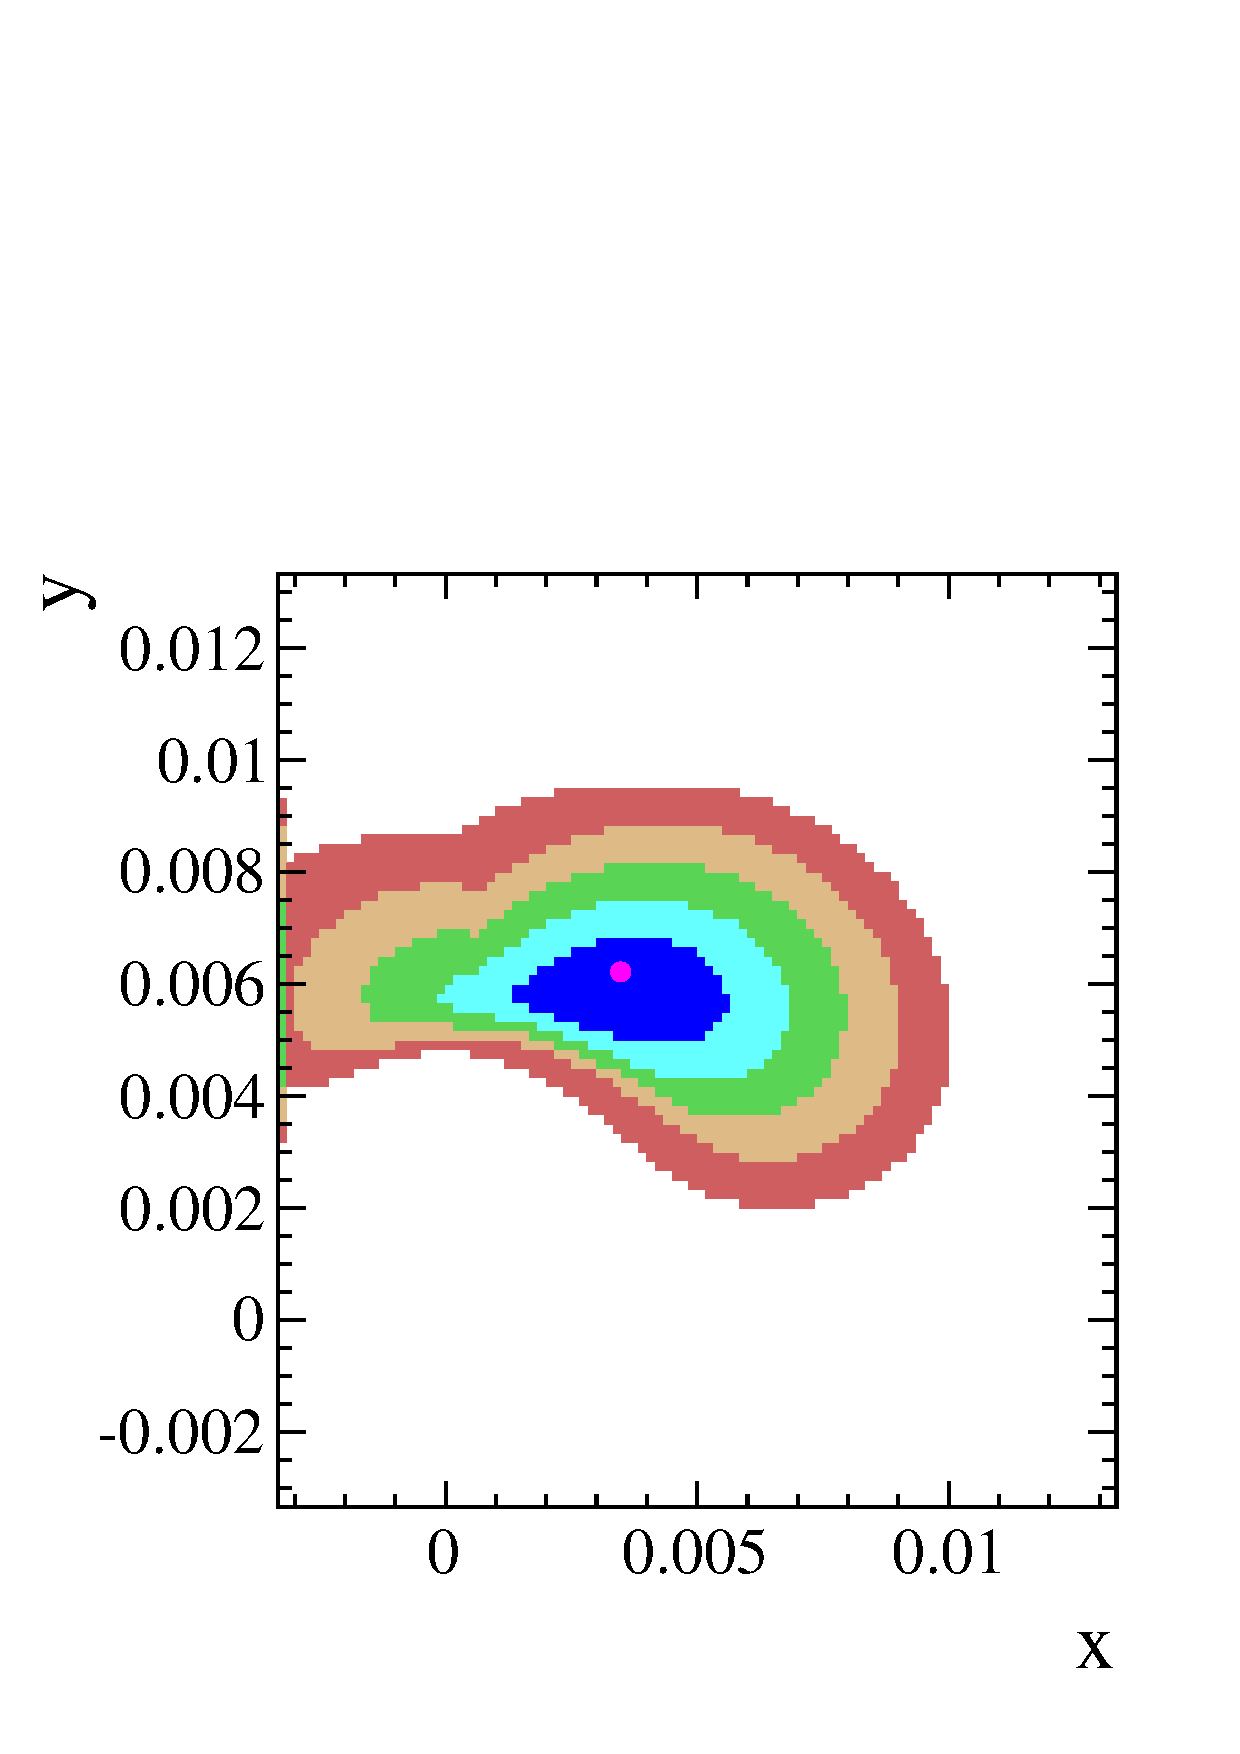
\includegraphics[width=\textwidth]{finalplot_allcpv_no_belle_babar_graph_hfag_agamma.pdf}
      \caption{Two dimensional error ellipses for x and y from fit excluding Belle and BaBar $K\pi$ results. Does not include latest $A_\Gamma$ result of LHCb.}
      \label{fig:xy_all_cpv_no_agamma}
    \end{subfigure}%
    \hspace{2mm}
    \begin{subfigure}[b]{0.4\textwidth}
      \centering
      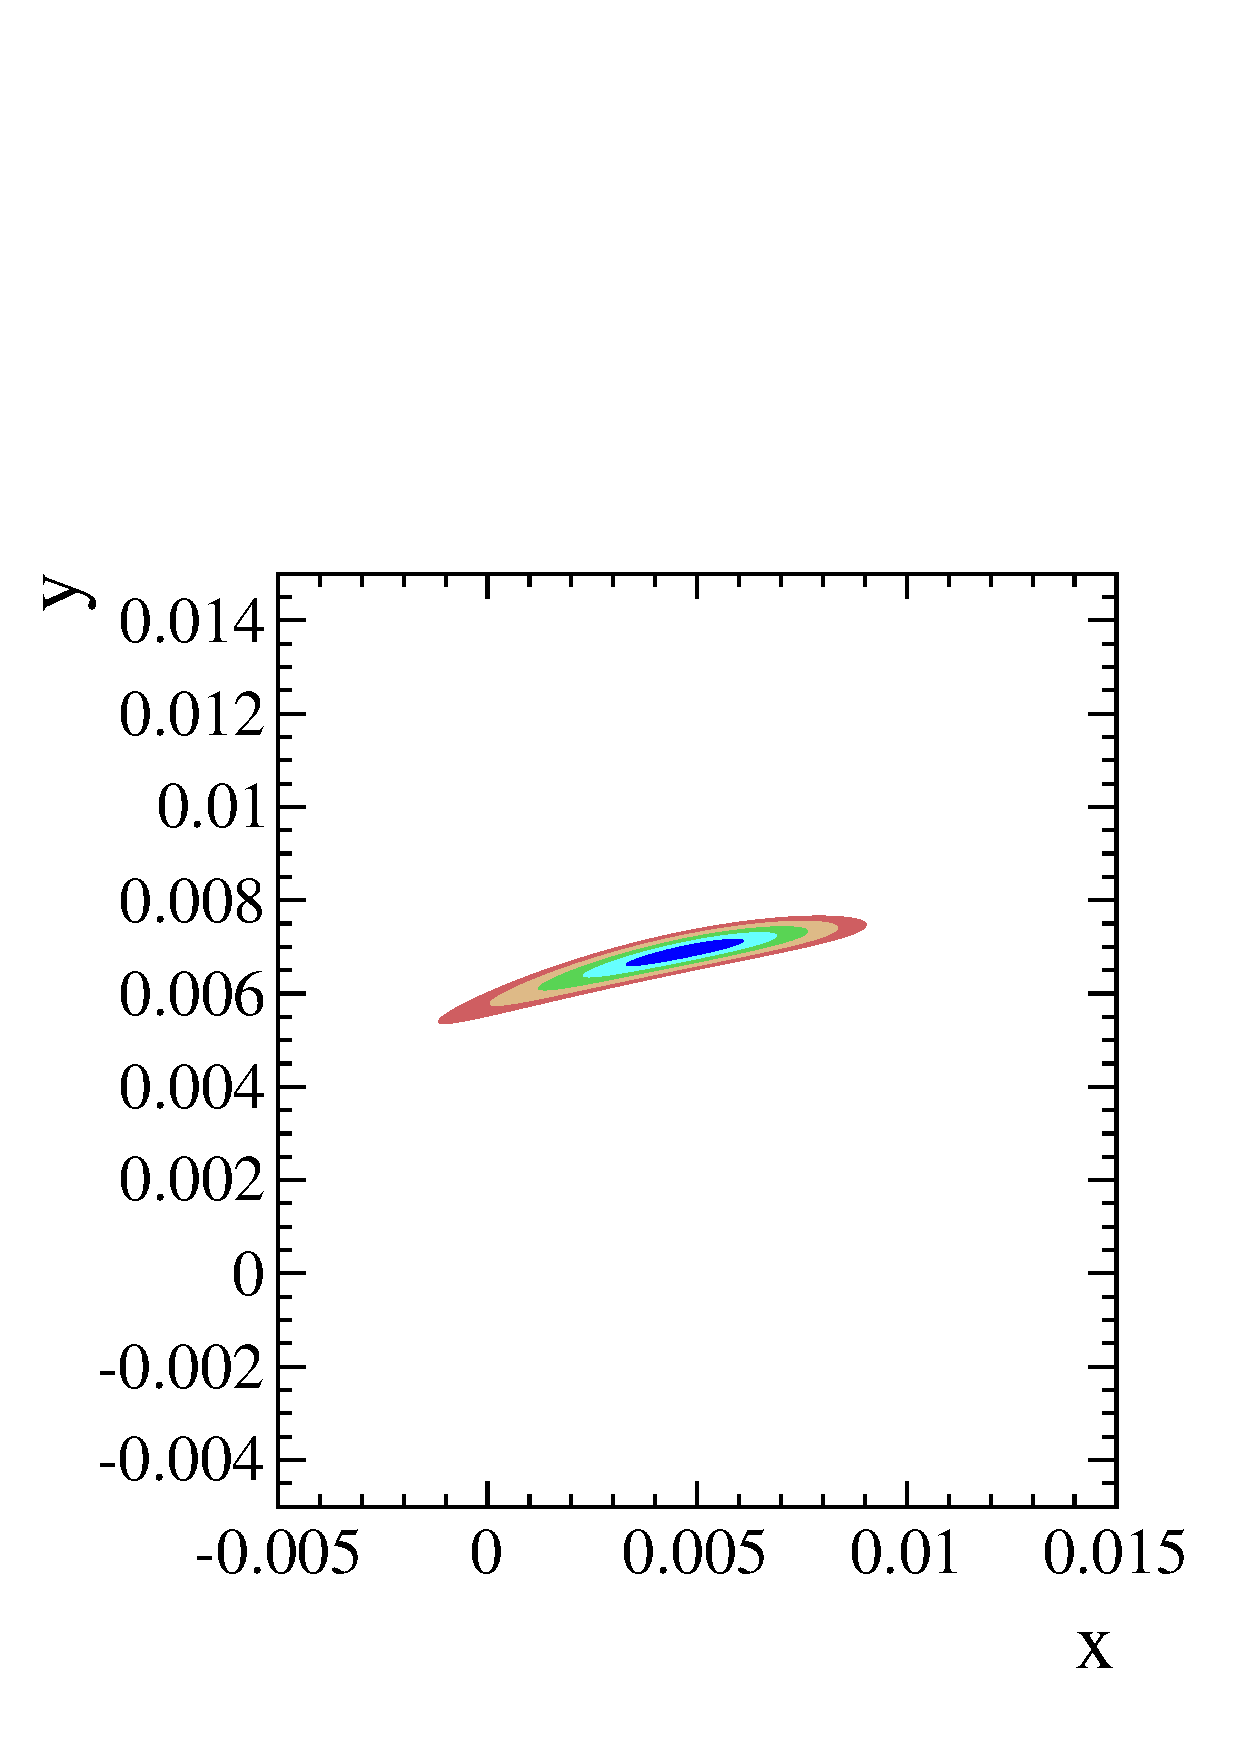
\includegraphics[width=\textwidth]{finalplot_allcpv_no_belle_babar_graph_lhcb_agamma.pdf}
      \caption{Two dimensional error ellipses for x and y from fit excluding Belle and BaBar $K\pi$ results. Include latest $A_\Gamma$ result of LHCb.}
      \label{fig:xy_all_cpv_with_agamma}
    \end{subfigure}%
    \\
    
%%%%%%%%%
    %\hspace{2mm}
    \begin{subfigure}[b]{0.4\textwidth}
      \centering
      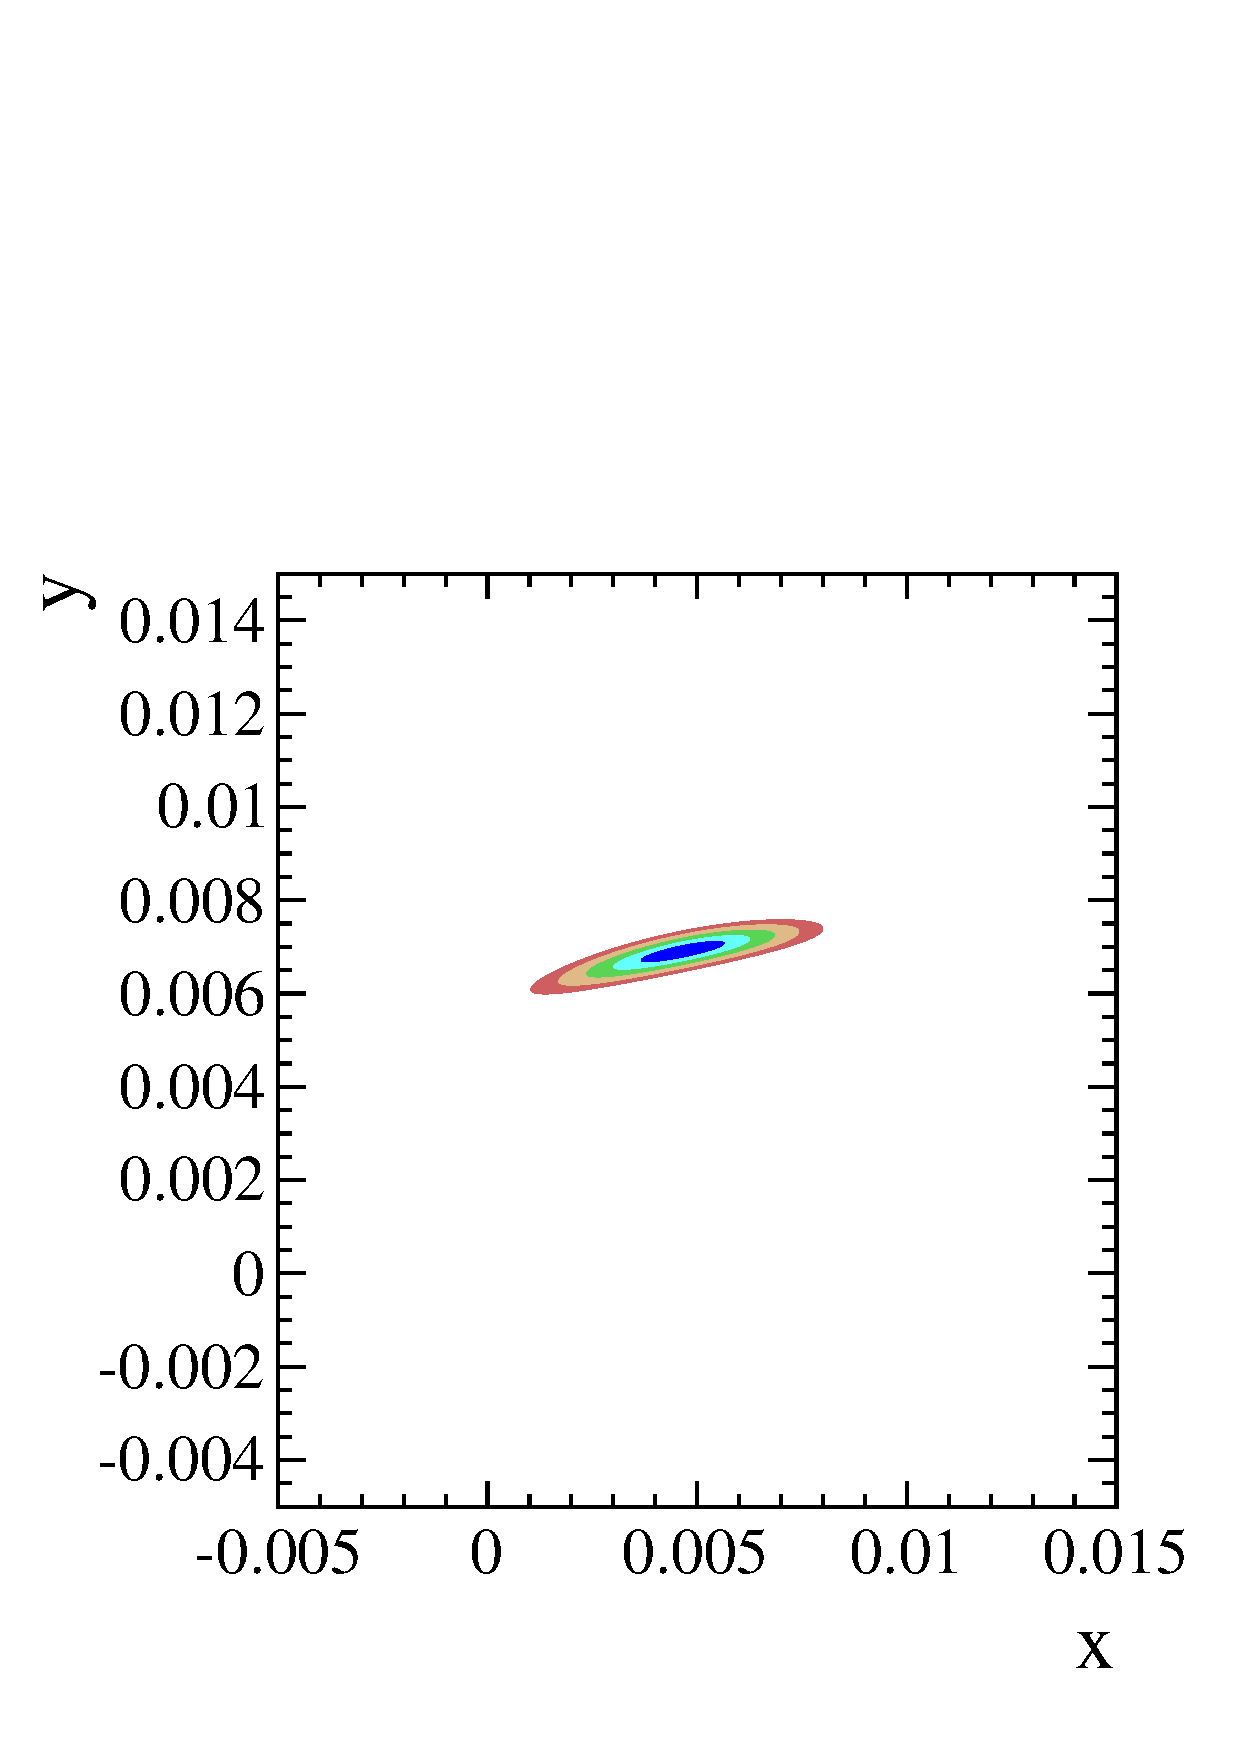
\includegraphics[width=\textwidth]{finalplot_allcpv_no_belle_babar_cdf_graph_hfag_agamma.pdf}
      \caption{Two dimensional error ellipses for x and y from fit excluding Belle, BaBar and CDF $K\pi$ results. Does not include latest $A_\Gamma$ result of LHCb.}
      \label{fig:xy_all_cpv_no_agamma}
    \end{subfigure}%
    \hspace{2mm}
    \begin{subfigure}[b]{0.4\textwidth}
      \centering
      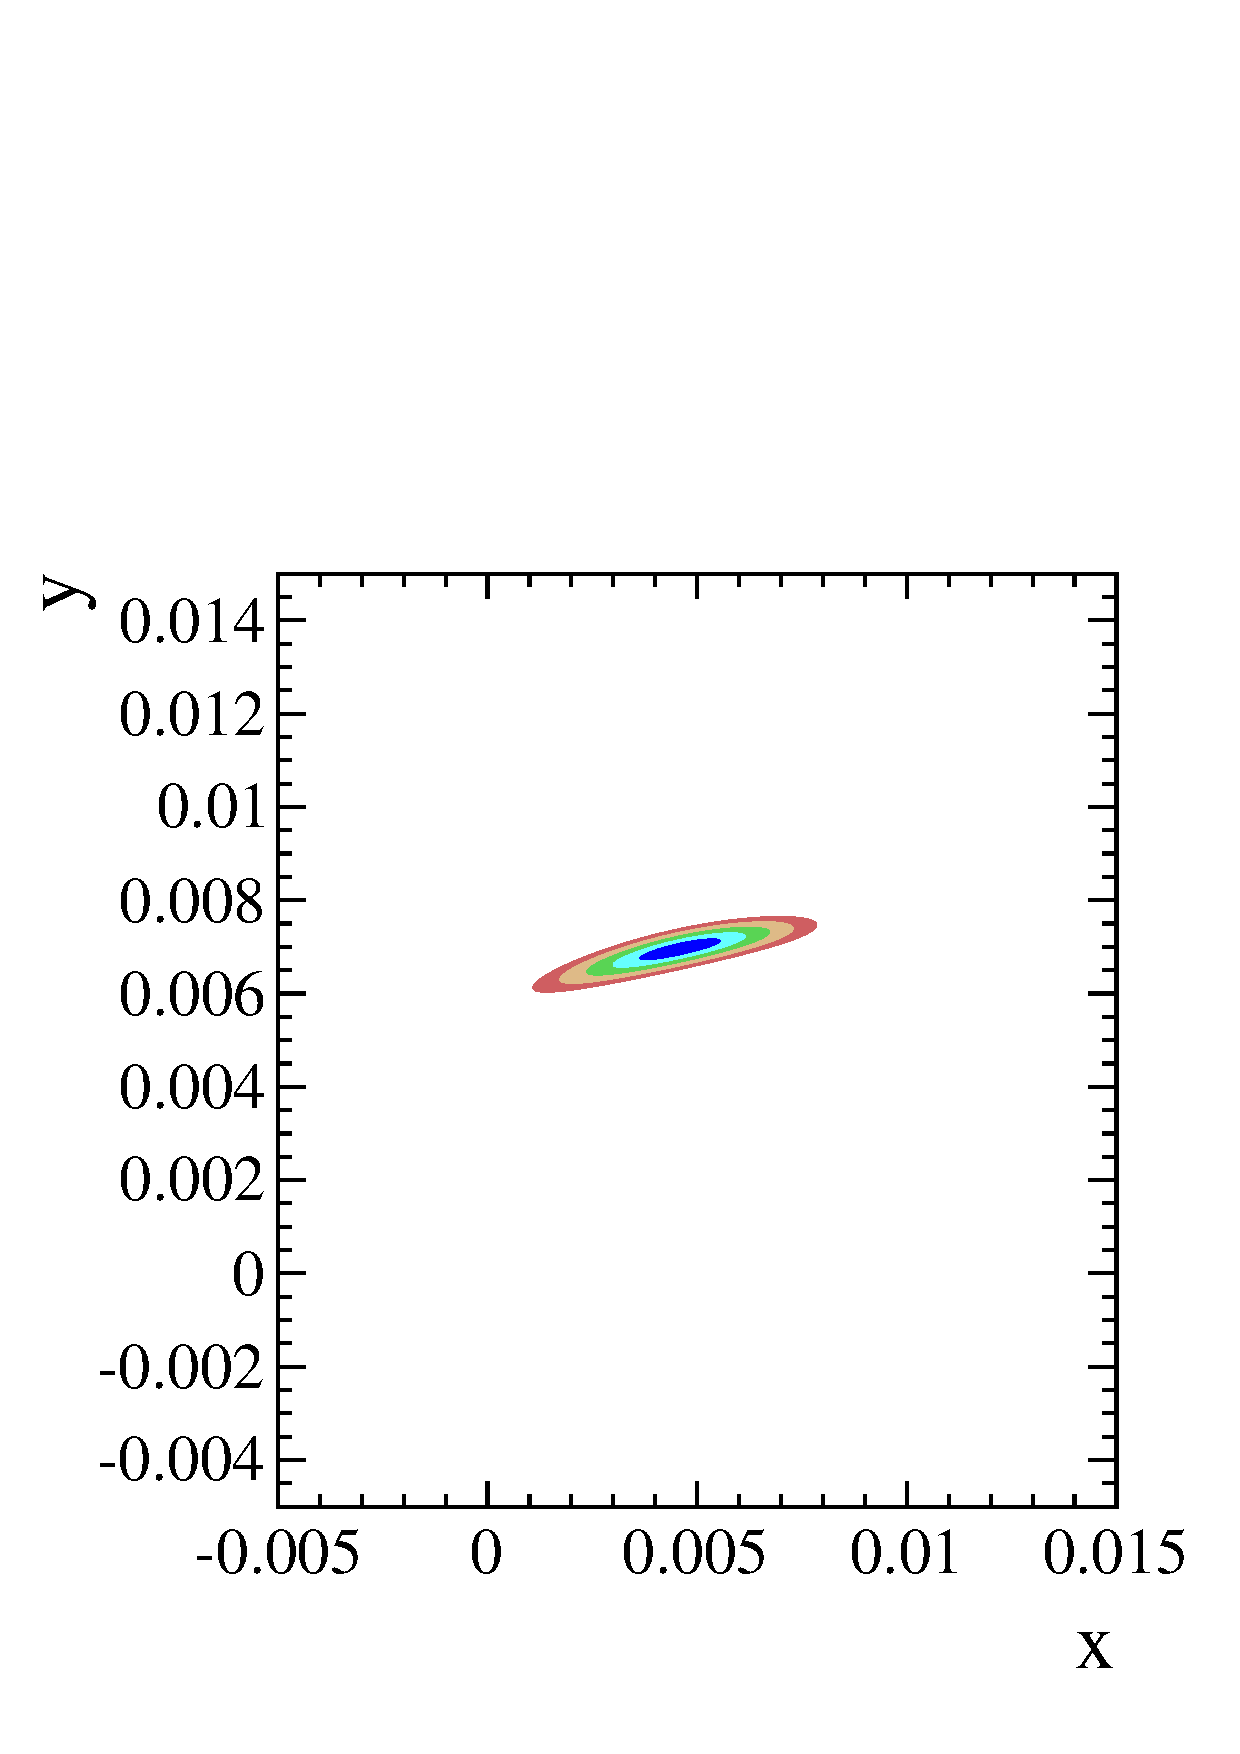
\includegraphics[width=\textwidth]{finalplot_allcpv_no_belle_babar_cdf_graph_lhcb_agamma.pdf}
      \caption{Two dimensional error ellipses for x and y from fit excluding Belle, BaBar and CDF $K\pi$ results. Include latest $A_\Gamma$ result of LHCb.}
      \label{fig:xy_all_cpv_with_agamma}
    \end{subfigure}%
    %\vspace*{-1.0cm}
  \end{center}
  \caption{Two dimensional error ellipses of fit for All CPV including differing sets of data for $x$ vs $y$. The biggest differences come from including the CDF result, which elongates the error ellipses. The differing colors represent the 1-5$\sigma$ contours.}
  \label{fig:xy_all_variations}
\end{figure}

%%%%%%%%%%%%%%%% Q/P %%%%%%%%%%%%%%%%%%%%%%%%%%%%%%%%%%%%
\begin{figure}[tb]
  \begin{center}
    \begin{subfigure}[b]{0.4\textwidth}
      \centering
      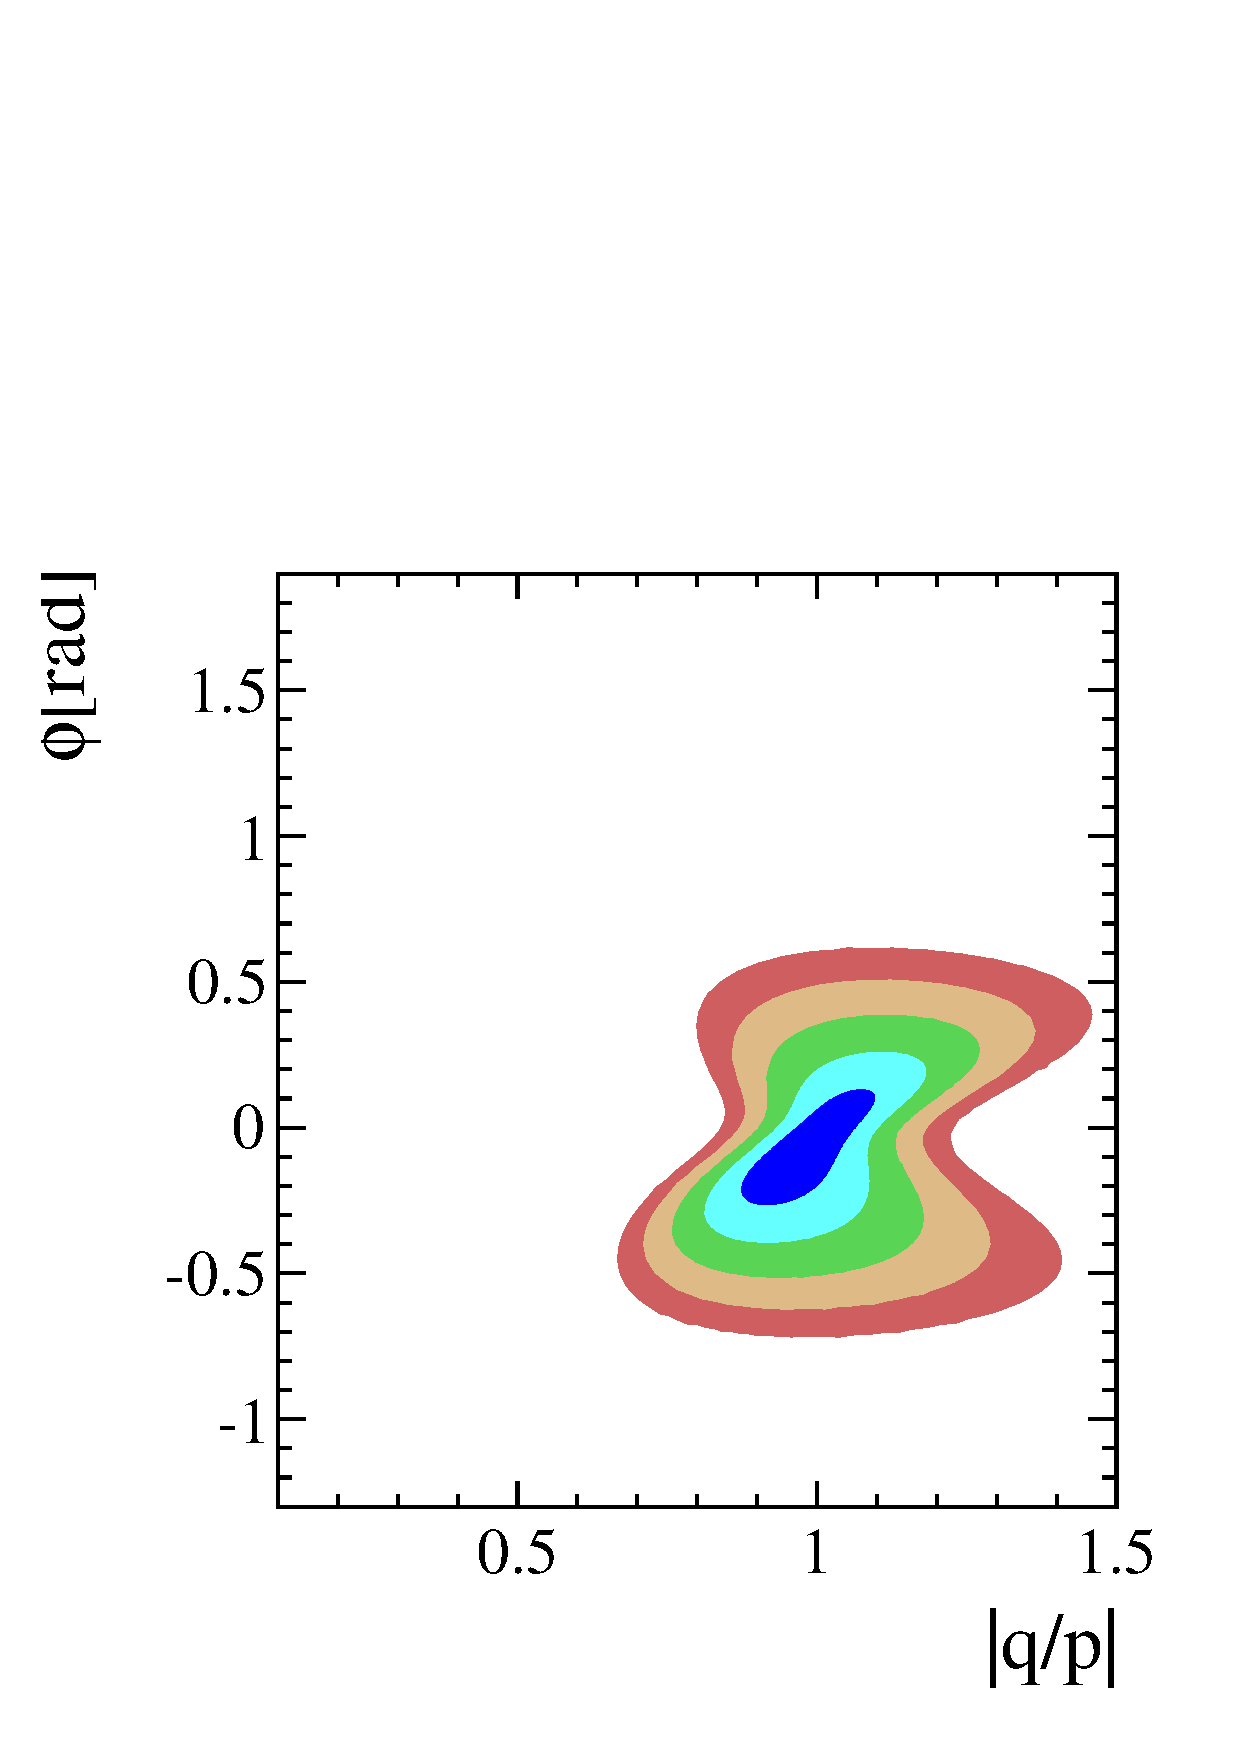
\includegraphics[width=\textwidth]{finalplot_allcpv_no_belle_babar_graph_qop_phi_hfag_agamma.pdf}
      \caption{Two dimensional error ellipses for x and y from fit excluding Belle and BaBar $K\pi$ results. Does not include latest $A_\Gamma$ result of LHCb.}
      \label{fig:xy_all_cpv_no_agamma}
    \end{subfigure}% 
    \hspace{2mm}
    \begin{subfigure}[b]{0.4\textwidth}
      \centering
      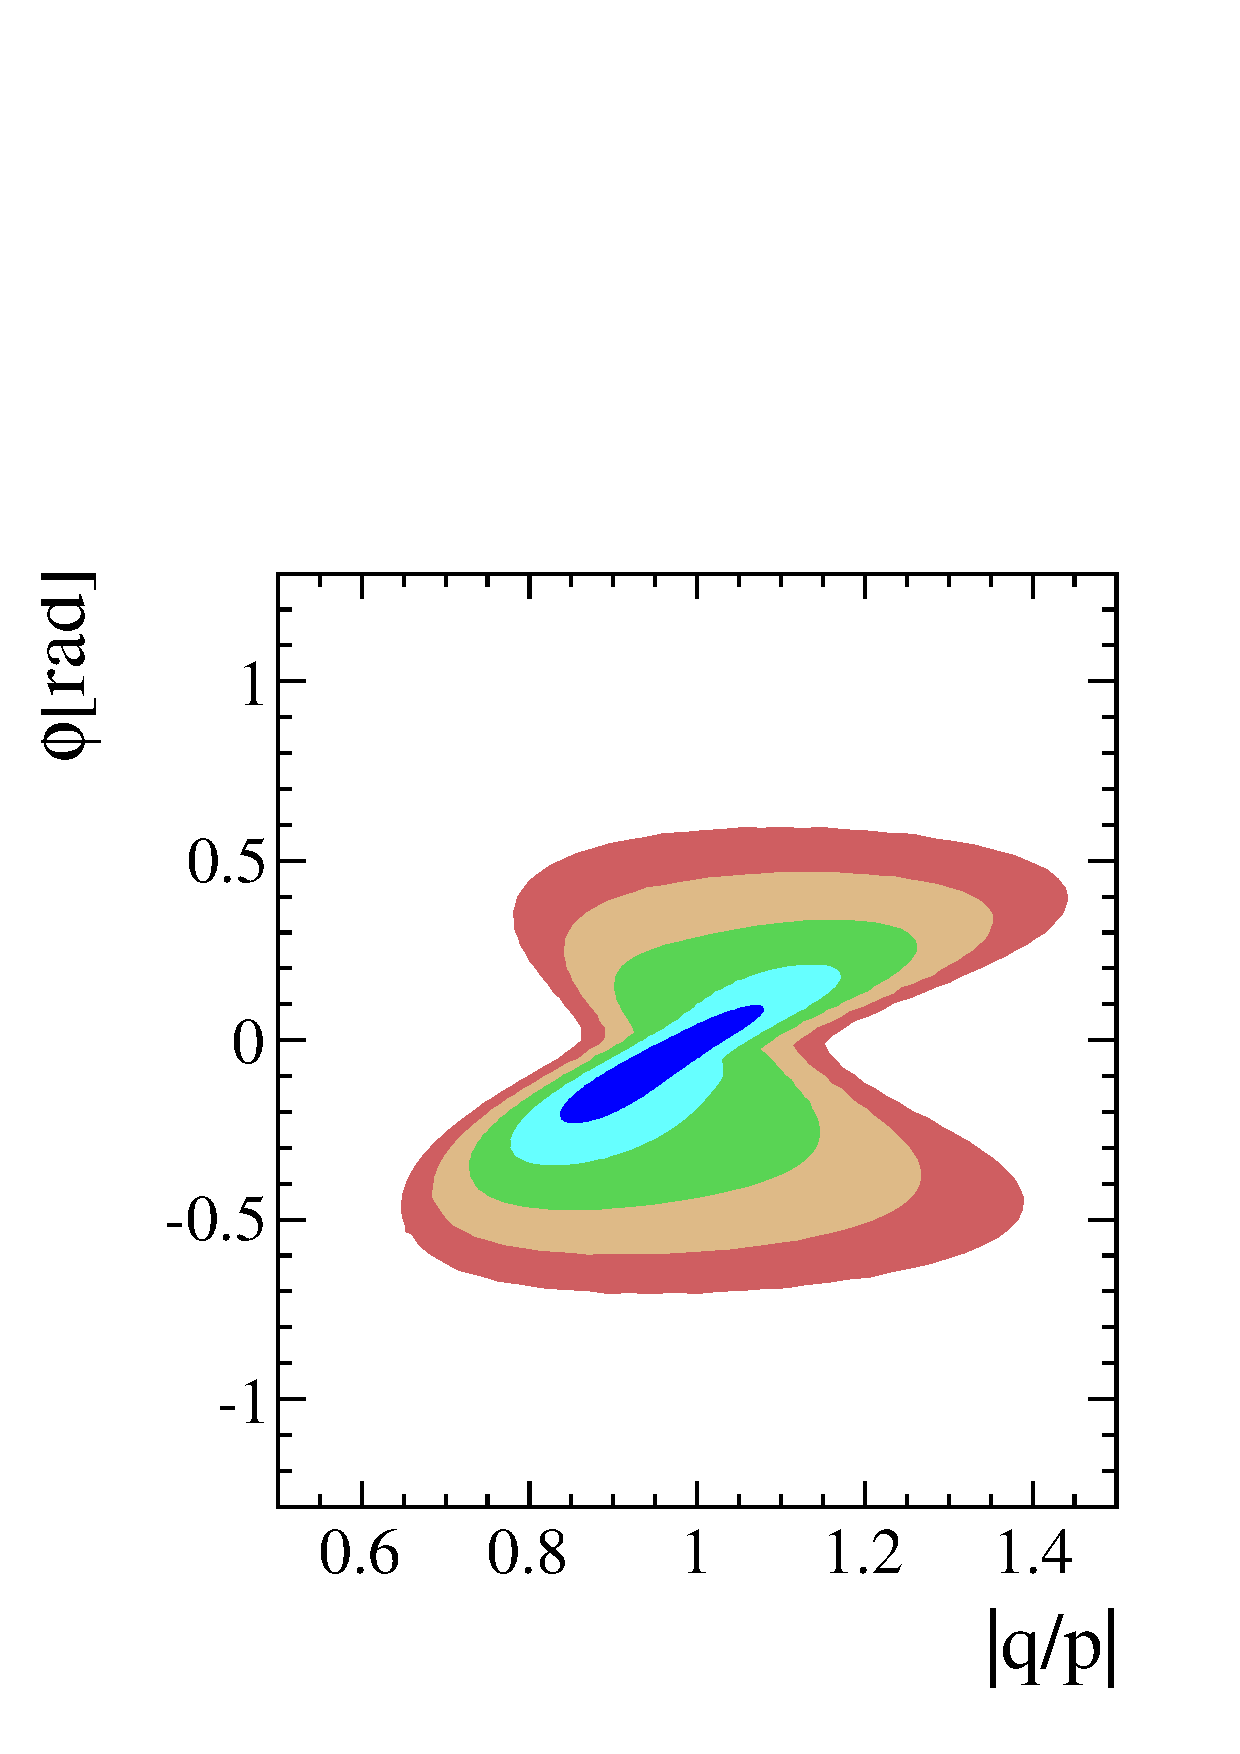
\includegraphics[width=\textwidth]{finalplot_allcpv_no_belle_babar_graph_qop_phi_lhcb_agamma.pdf}
      \caption{Two dimensional error ellipses for x and y from fit excluding Belle and BaBar $K\pi$ results. Include latest $A_\Gamma$ result of LHCb.}
      \label{fig:xy_all_cpv_with_agamma}
    \end{subfigure}%
%%%%%%%%%
        \\
    \begin{subfigure}[b]{0.4\textwidth}
      \centering
      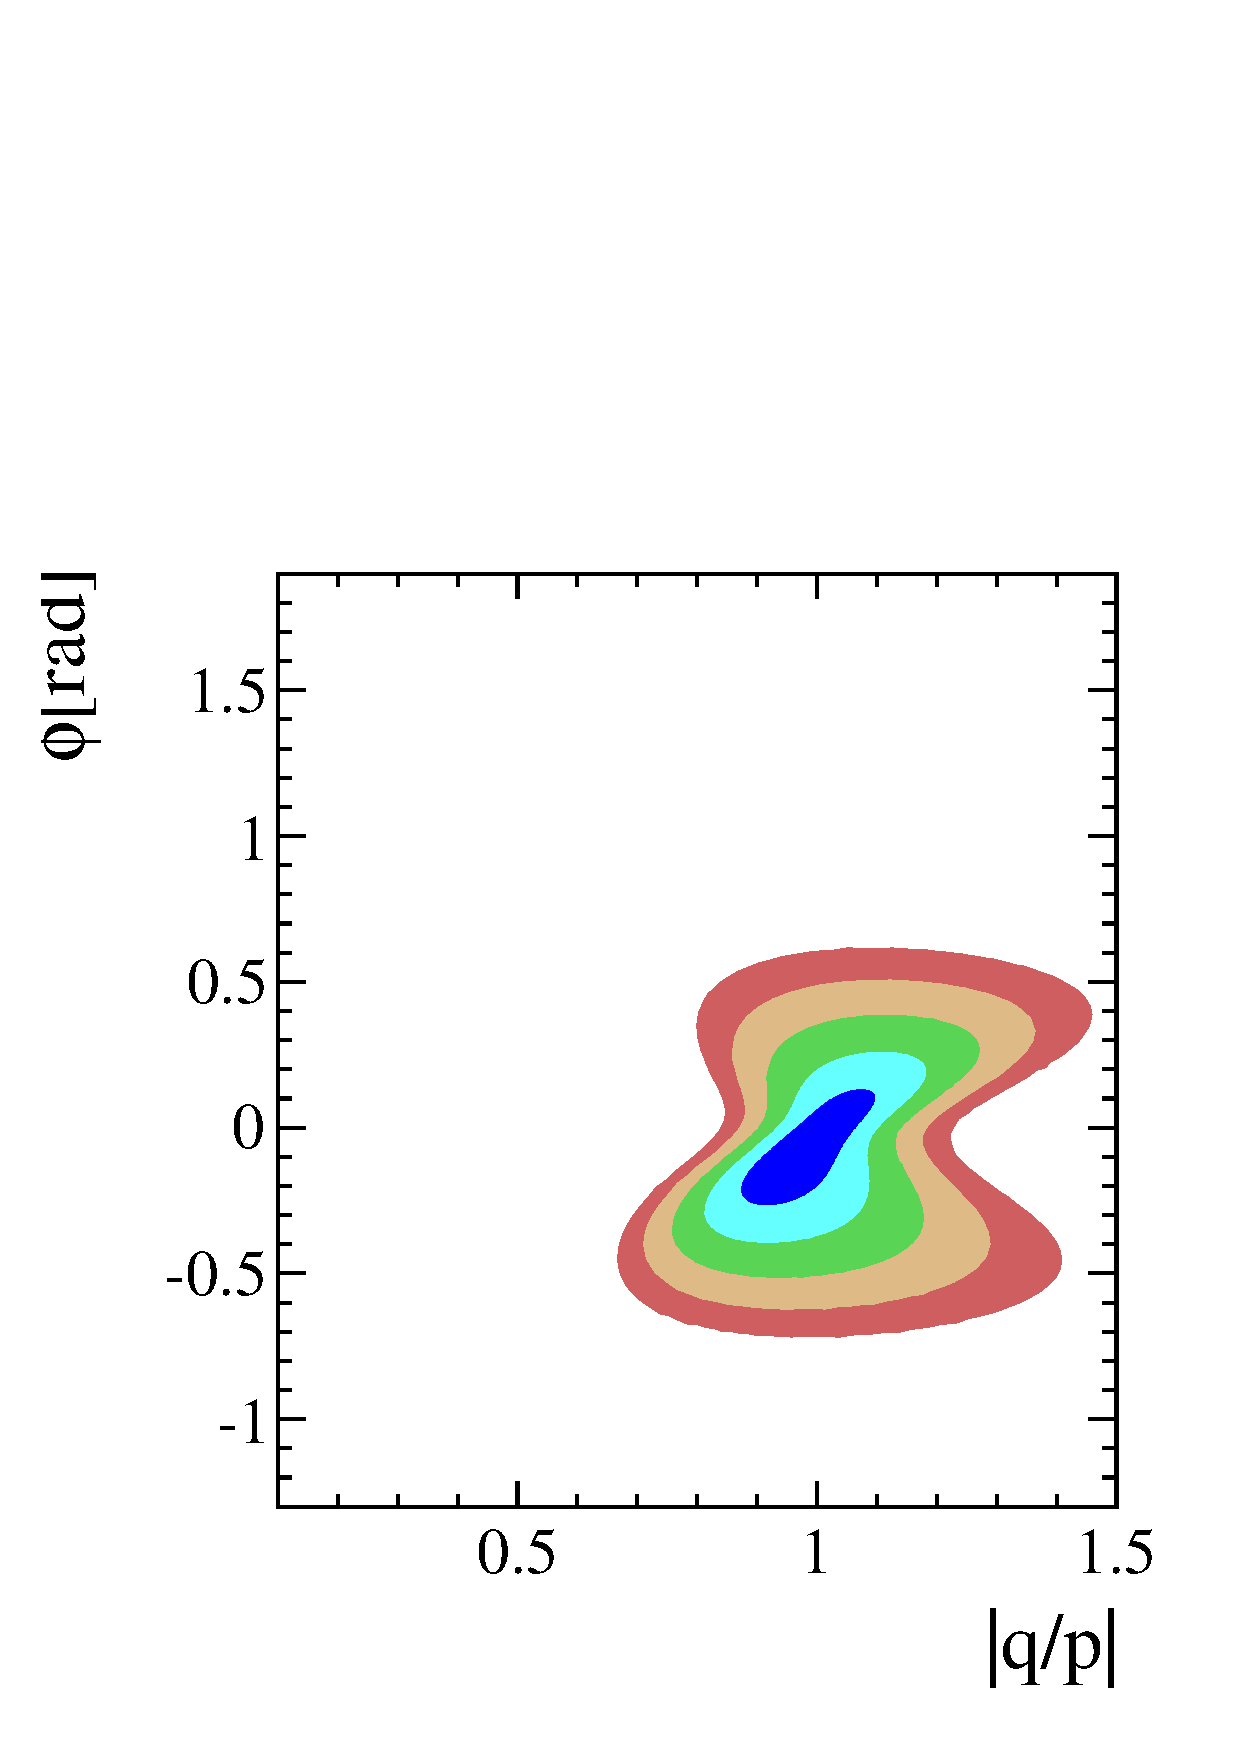
\includegraphics[width=\textwidth]{finalplot_allcpv_no_belle_babar_cdf_graph_qop_phi_hfag_agamma.pdf}
      \caption{Two dimensional error ellipses for x and y from fit excluding Belle, BaBar and CDF $K\pi$ results. Does not include latest $A_\Gamma$ result of LHCb.}
      \label{fig:xy_all_cpv_no_agamma}
    \end{subfigure}%
    \hspace{2mm}
    \begin{subfigure}[b]{0.4\textwidth}
      \centering
      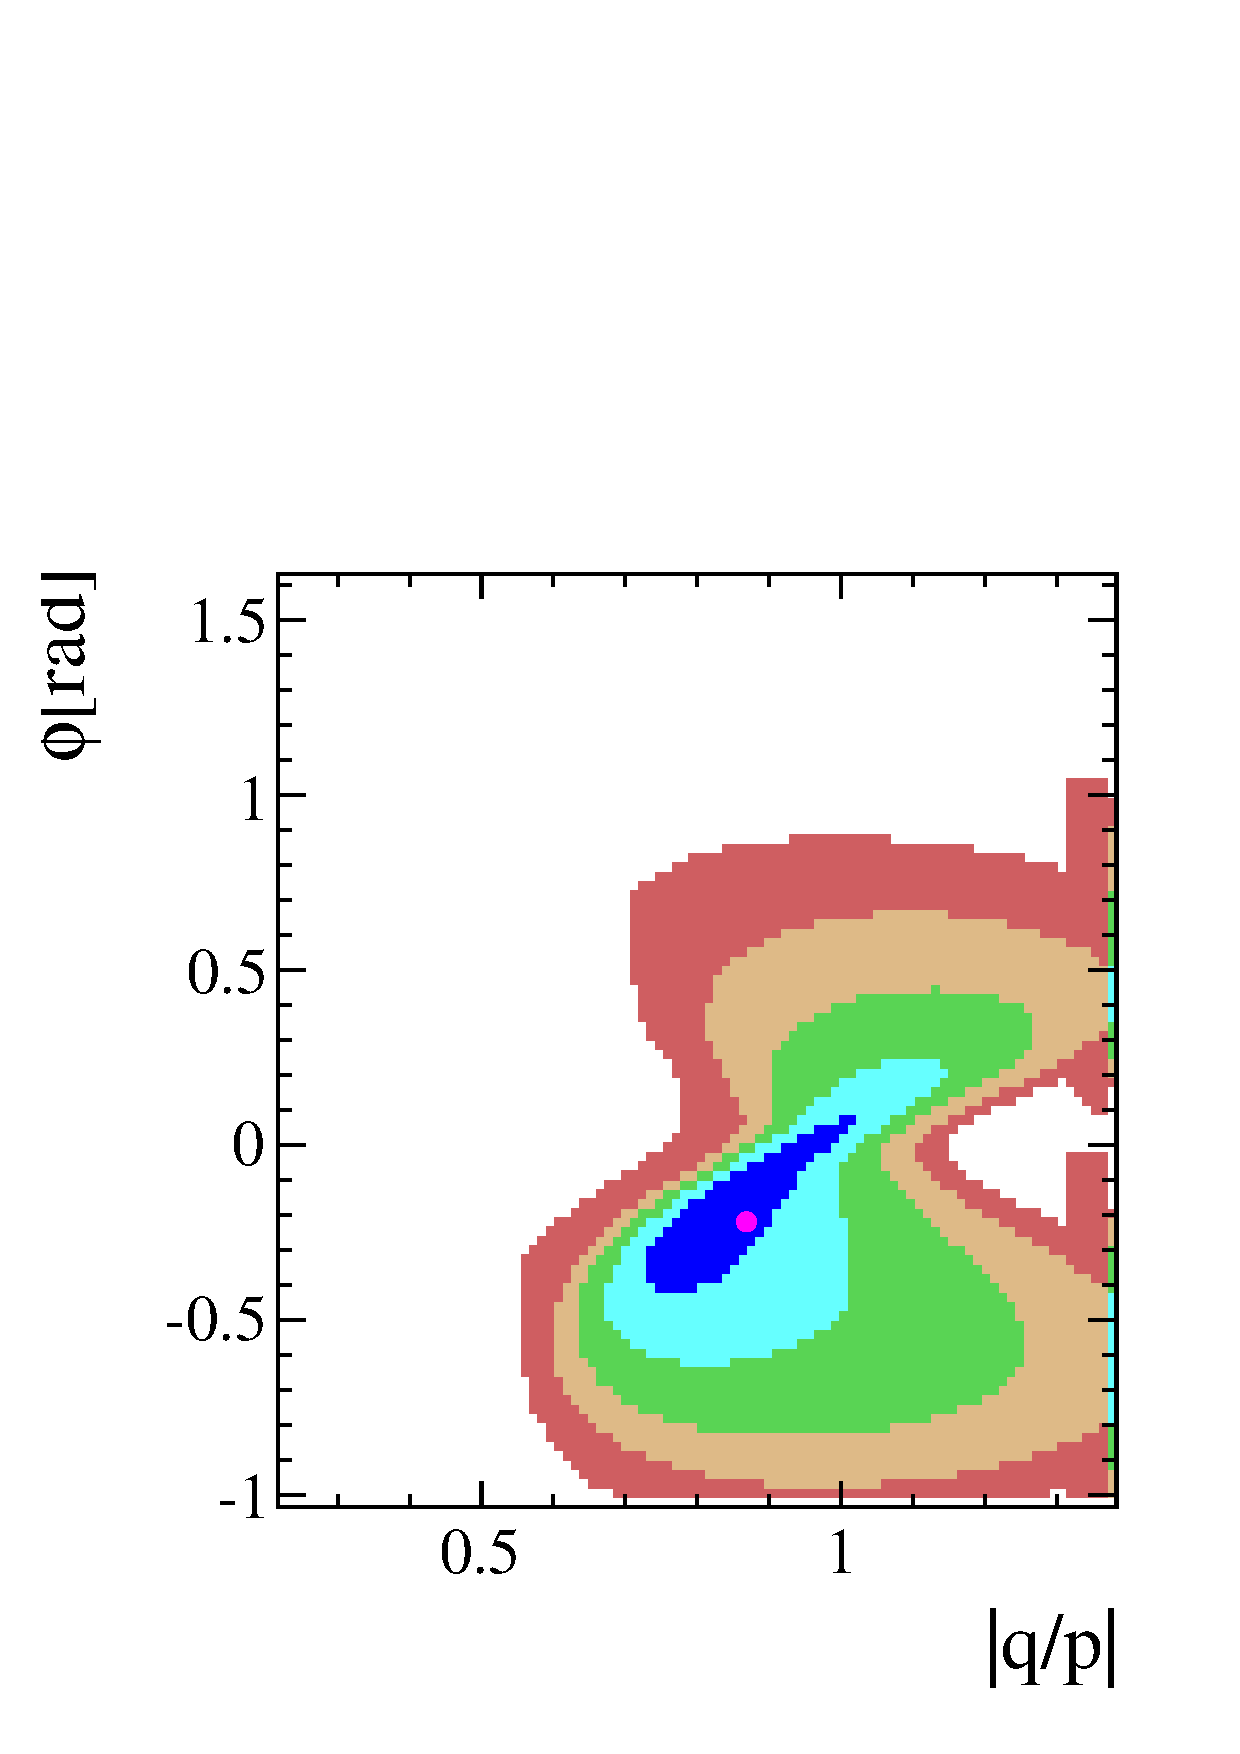
\includegraphics[width=\textwidth]{finalplot_allcpv_no_belle_babar_cdf_graph_qop_phi_lhcb_agamma.pdf}
      \caption{Two dimensional error ellipses for x and y from fit excluding Belle, BaBar and CDF $K\pi$ results. Include latest $A_\Gamma$ result of LHCb.}
      \label{fig:xy_all_cpv_with_agamma}
    \end{subfigure}%
    %\vspace*{-1.0cm}
  \end{center}
  \caption{Two dimensional error ellipses of fit for All CPV including differing sets of data for $\phi$ vs $q/p$. The biggest differences come from including the CDF result, which elongates the error ellipses. The differing colors represent the 1-5$\sigma$ contours.}
  \label{fig:xy_all_variations}
\end{figure}

%\subsection{All CP Violation Allowed, Fit for $x_{12},y_{12},\phi_{12}$}
%Table~\ref{table:allcpv_output_table_alex} lists the results for the All CPV allowed fit with the substitution of $x$ and $y$ for the underying parameters $x_{12},y_{12}$ and $\phi_{12}$. 
%\begin{table}[htdp]
%\begin{tiny}

\begin{center}
\resizebox{16cm}{!} {
\begin{tabular}{|c||c||c||c||c|}
\hline
& All Measurements & No Belle, BaBar& No Belle, BaBar, $A_{\Gamma\text{ LHCb}}$ & No Belle, BaBar, CDF,$A_{\Gamma\text{ LHCb}}$ \\ \hline

$x_{12}(\times10^{-3})$&$ 3.789\pm1.627$  & $4.842\pm1.693$&$4.842\pm1.693$ & $4.853\pm1.694$\\ \hline

$y_{12}(\times10^{-3})$&$ 6.365\pm 0.953$  &$6.851\pm0.099$ & $6.851\pm 0.994$&$6.863\pm0.994$ \\ \hline

$\delta_{K\pi}(\times10^{-1})[\text{rad}]$&$1.855\pm 2.523$ & $3.237\pm1.949$& $3.237\pm1.949$&$3.191\pm1.950$ \\ \hline

$\phi_{12}(\times10^{-2})[\text{rad}]$&$-0.304\pm4.277$ &$-0.210\pm3.416$ & $-0.210\pm3.416$&$-0.249\pm3.380$ \\\hline

$R_D^-(\times10^{-3})$&$3.501\pm0.038$ & $3.556\pm0.043$& $3.556\pm0.043$& $3.556\pm0.043$\\ \hline

$R_D^+(\times10^{-3})$& $3.505\pm0.038$& $3.558\pm0.043$& $3.558\pm0.043$& $3.558\pm0.043$\\ \hline

$\chi^2/ndf$& 50.73/27&  19.5825/15& 19.5825/15& 8.62343/12\\ \hline

\end{tabular}
}
\end{center}
\caption{Output of the All CP Violation allowed global fit when fitting for the 
underlying parameters $x_{12}$ and $y_{12}$. Different Columns list 
differing subsets of data included in the fit.}
\label{table:allcpv_output_table_alex}
%\end{tiny}
\end{table}%

